% This is samplepaper.tex, a sample chapter demonstrating the
% LLNCS macro package for Springer Computer Science proceedings;
% Version 2.21 of 2022/01/12
%
\documentclass[runningheads]{llncs}
%
\usepackage[T1]{fontenc}
% T1 fonts will be used to generate the final print and online PDFs,
% so please use T1 fonts in your manuscript whenever possible.
% Other font encondings may result in incorrect characters.
%
\usepackage{graphicx}
% Used for displaying a sample figure. If possible, figure files should
% be included in EPS format.
%
\usepackage{cite}
\usepackage{amsmath,amssymb,amsfonts}
\usepackage{algorithmic}
\usepackage{textcomp}
\usepackage{xcolor}
\usepackage{booktabs}

% for highlighted texts with color
\usepackage{color}
\usepackage{soul}
\definecolor{codebox-color}{rgb}{0.925, 0.925, 0.925}
\sethlcolor{codebox-color}

%
%\makeatletter
%\def\SOUL@hlpreamble{%
%    \setul{}{3.5ex}% increased by 1ex
%    \let\SOUL@stcolor\SOUL@hlcolor
%    \dimen@\SOUL@ulthickness
%    \dimen@i=-.75ex % increased by -0.25ex
%    \advance\dimen@i-.5\dimen@
%    \edef\SOUL@uldepth{\the\dimen@i}%
%    \let\SOUL@ulcolor\SOUL@stcolor
%    \SOUL@ulpreamble
%}
%\makeatother

\newcommand*{\codebox}[1]{{\ttfamily\hyphenchar\font=45\relax\hl{~#1~}}}

\newcommand{\cloudonlycolor}[1]{{\sethlcolor{orange!35!}\hl{#1}}}
\newcommand{\cloudedgecolor}[1]{{\sethlcolor{green!35!}\hl{#1}}}

\usepackage{lineno}
\usepackage{breqn}

% for subscript and superscript in normal text
\usepackage{fixltx2e}

% for heterogeneity table
\usepackage{array,tabularx}
\newcolumntype{Y}{>{\centering\arraybackslash}X}
\usepackage{booktabs}

% for empty set symbol
\usepackage{amssymb}
\let\oldemptyset\emptyset
\let\emptyset\varnothing

% for table
 \usepackage{array,multirow,graphicx}
 \usepackage{float}

% for side by side figures
\usepackage{subcaption}
\usepackage{array}
\usepackage{booktabs} 

% for strikethrough
\usepackage{soul}

\usepackage{listings}

\usepackage{pgfplots,pgfplotstable}
\usetikzlibrary{patterns.meta}
\usetikzlibrary{positioning,fit,arrows.meta,backgrounds}
\usetikzlibrary{backgrounds}
% Pie chart drawing library 
\usepackage{pgf-pie}

% for cell colors in tables
\usepackage{xcolor,colortbl}

% for double line in table
\usepackage{hhline}

% for table font
%\usepackage{tgschola}            % TeX Gyre Schola (serif)
%\usepackage[condensed]{tgschola} % condensed shape
%\usepackage{tgheros}
%\usepackage[condensed]{tgheros}

\pgfplotsset{compat=newest}

% for spacing between sections
%\usepackage[pagestyles]{titlesec}
% Reduce space before and after section headings
%\titlespacing{\section}{0pt}{*0.8}{*0.3}  % {left}{before}{after}
%\titlespacing{\subsection}{0pt}{*0.6}{*0.2}
%\titlespacing{\subsubsection}{0pt}{*0.5}{*0.1}

% to show figures in pdf format
\usepackage{graphicx}

% for box plot
\usepgfplotslibrary{colorbrewer}
\usetikzlibrary{pgfplots.statistics, pgfplots.colorbrewer}
\usepackage{pgfplotstable}
\usepackage{filecontents}
\pgfplotsset{compat = 1.15, cycle list/Set1-8} 

\begin{filecontents*}{data.csv}
102.2, 103.4, 203.1, 102.7, 103.1, 41.4, 102.5
122.2, 123.7, 63.1, 223.1, 122.4, 122.6, 123.4
143.9, 144.2, 144.3, 243.0, 182.4, 143.5, 82.6
165.8, 165.4, 263.4, 165.2, 164.7, 163.9, 167.5
\end{filecontents*}


\begin{filecontents*}{data-numoftuples.csv}
102.6, 103.1, 203.1, 102.7, 103.1, 41.4, 202.3, 105.5, 104.4, 106.6, 104.9, 104.6 %100
120.2, 125.9, 121.3, 123.8, 221.5, 121.7, 43.4, 123.6, 121.8, 111.7, 123.5, 121.1 %500
127.3, 126.2, 128.4, 124.6, 148.3, 149.2, 225.1, 135, 51, 132, 115, 135 %1000
152.3, 193.2, 199.7, 210.3, 183.7, 209.2, 150.5, 216.5, 142.4, 140.1, 116.1, 148.8 %5000
\end{filecontents*}

\begin{filecontents*}{data-numoftuples-topdown.csv}
106.7, 105.8, 107.7, 104.2, 104.3, 106.5, 204.7, 105.9, 105.3, 104.1, 105.0, 107.6 %100
123.3, 121.4, 120.0, 123.1, 120.0, 220.5, 121.9, 122.7, 120.6, 120.6, 119.1, 124.2 %500
128.5, 132.3, 132.1, 225.2, 128.8, 133.4, 125.7, 123.1, 127.6, 125.6, 222.3, 138.4 %1000
145.2, 201.3, 157.4, 195.6, 191.3, 184.4, 133.3, 148.4, 176.6, 184.0, 199.9, 206.6 %5000
\end{filecontents*}

\begin{filecontents*}{data-numoftuples-bottomtop.csv}
102.6, 103.1, 203.1, 102.7, 103.1, 41.4, 202.3, 105.5, 104.4, 106.6, 104.9, 104.6 %100b
106.7, 105.8, 107.7, 104.2, 104.3, 106.5, 204.7, 105.9, 105.3, 104.1, 105.0, 107.6 %100t
120.2, 125.9, 121.3, 123.8, 221.5, 121.7, 43.4, 123.6, 121.8, 111.7, 123.5, 121.1 %500b
123.3, 121.4, 120.0, 123.1, 120.0, 220.5, 121.9, 122.7, 120.6, 120.6, 119.1, 124.2 %500t
127.3, 126.2, 128.4, 124.6, 148.3, 149.2, 225.1, 135, 51, 132, 115, 135 %1000b
128.5, 132.3, 132.1, 225.2, 128.8, 133.4, 125.7, 123.1, 127.6, 125.6, 222.3, 138.4 %1000t
152.3, 193.2, 199.7, 210.3, 183.7, 209.2, 150.5, 216.5, 142.4, 140.1, 116.1, 148.8 %5000b
145.2, 201.3, 157.4, 195.6, 191.3, 184.4, 133.3, 148.4, 176.6, 184.0, 199.9, 206.6 %5000t
\end{filecontents*}


% define colors for charts

\definecolor{dorange}{RGB}{204,102,0}
\definecolor{cyan}{RGB}{0,153,255}

\definecolor{blue0}{RGB}{0,0,150}
\definecolor{blue1}{RGB}{30,60,255}
\definecolor{blue2}{RGB}{60,120,255}
\definecolor{blue3}{RGB}{0,184,230}
\definecolor{blue4}{RGB}{194,194,255}
\definecolor{blue5}{RGB}{38,77,115}

\tikzstyle{bar chart}=[
    chart,
    bar width/.code={
        \pgfmathparse{##1/2}
        \global\let\bar@w\pgfmathresult
    },
    bar/.style={very thick, draw=white},
    bar label/.style={font={\bf\small},anchor=north},
    bar value/.style={font={\footnotesize}},
    bar width=.75,
]

\makeatletter

% for highlighted texts with color


\tikzstyle{chart}=[
    legend label/.style={font={\scriptsize},anchor=west,align=left},
    legend box/.style={rectangle, draw, minimum size=5pt},
    axis/.style={black,semithick,->},
    axis label/.style={anchor=east,font={\tiny}},
]

\tikzstyle{bar chart}=[
    chart,
    bar width/.code={
        \pgfmathparse{##1/2}
        \global\let\bar@w\pgfmathresult
    },
    bar/.style={very thick, draw=white},
    bar label/.style={font={\bf\small},anchor=north},
    bar value/.style={font={\footnotesize}},
    bar width=.75,
]

\tikzstyle{pie chart}=[
    chart,
    slice/.style={line cap=round, line join=round, very thick,draw=white},
    pie title/.style={font={\bf}},
    slice type/.style 2 args={
        ##1/.style={fill=##2},
        values of ##1/.style={}
    },
    slice type pattern/.style 2 args={
        ##1/.style={pattern=##2},
        values of ##1/.style={}
    }
]

\pgfdeclarelayer{background}
\pgfdeclarelayer{foreground}
\pgfsetlayers{background,main,foreground}
\usetikzlibrary{patterns}



\newcommand{\legend}[2][]{
    \begin{scope}[#1]
    \path
        \foreach \n/\s in {#2}
            {
                  ++(0,-10pt) node[\s,legend box] {} +(5pt,0) node[legend label] {\n}
            }
    ;
    \end{scope}
}

\usepackage{scalerel}
\usepackage{tikz}
\usetikzlibrary{svg.path}


% for custom listing for yaml
\lstdefinelanguage{CustomYAML}{
    morekeywords={datagen, period, duration, dataset, distribution, rate, pattern, skew, network, topology, depth, branching, heterogeneity, latency, bandwidth, host, ports, cpu, memory, storage, n1, n2, n3, n4, n5},
    sensitive=false,
    morecomment=[l]{\#},
    morestring=[b]",
    morestring=[b]',
    literate=
      {:}{{\textbf{:}}}1
      {,}{{\textbf{,}}}1
      {-}{{\textbf{-}}}1
      {>}{{\textbf{>}}}1
      {|}{{\textbf{|}}}1
      {\ }{{\ }}1
      {~}{{\textbf{\textasciitilde}}}1
}

\lstdefinestyle{yamlstyle}{
    language=CustomYAML,
    basicstyle=\scriptsize\rmfamily,
    keywordstyle=\color{black}\bfseries,
    commentstyle=\color{gray}\itshape,
    stringstyle=\color{black},
    showstringspaces=false,
    breaklines=true,
    aboveskip=0pt,
    belowskip=0pt
}

\lstdefinelanguage{SQL}{
    morekeywords={
        SELECT, FROM, WHERE, AND, OR, INSERT, INTO, VALUES, UPDATE, SET, DELETE, CREATE, TABLE, INNER, JOIN, ON, AS, IN, GROUP, BY, HAVING, COUNT, WINDOW, TUMBLING
    },
    sensitive=false,
    morecomment=[l]--,
    morestring=[b]',
}

\lstdefinestyle{sqlstyle}{
    language=SQL,
    basicstyle=\ttfamily\scriptsize,
    keywordstyle=\color{blue}\bfseries,
    commentstyle=\color{gray}\itshape,
    stringstyle=\color{orange},
    showstringspaces=false,
    breaklines=true,
}

% for circled numbers in text
\newcommand*\circled[1]{%
  \tikz[baseline=(char.base)]{%
    \node[circle,draw,inner sep=0.6pt,font=\scriptsize] (char) {#1};%
  }%
}

% for dotted line in text
% Inline legend line (colored + patterned)
\newcommand{\inlineline}[1]{%
  \tikz[baseline=-0.6ex]\draw[#1,line cap=round] (0,0)--(1.8em,0);%
}



% If you use the hyperref package, please uncomment the following two lines
% to display URLs in blue roman font according to Springer's eBook style:
%\usepackage{color}
%\renewcommand\UrlFont{\color{blue}\rmfamily}
%\urlstyle{rm}
%
\begin{document}
%
% for spacing between sections
%\setlength{\parskip}{0pt} % Reduce paragraph spacing
%\renewcommand{\baselinestretch}{0.98} % Slightly reduce line spacing
%
%\makeatletter
%\renewcommand{\section}{\@startsection{section}{1}{\z@}%
%  {6pt plus 2pt minus 2pt} % Space before
%  {3pt plus 1pt minus 1pt} % Space after
%  {\normalfont\large\bfseries\boldmath
%                        \rightskip=\z@ \@plus 8em\pretolerance=10000 }}
%
%\renewcommand{\subsection}{\@startsection{subsection}{2}{\z@}%
%  {5pt plus 1pt minus 1pt}%
%  {2pt plus 1pt minus 1pt}%
%  {\normalfont\normalsize\bfseries\boldmath
%                        \rightskip=\z@ \@plus 8em\pretolerance=10000 }}
%
%\renewcommand{\subsubsection}{\@startsection{subsubsection}{3}{\z@}%
%  {4pt plus 1pt minus 1pt}%
%  {1pt plus 1pt minus 1pt}%
%  {\normalfont\small\bfseries\boldmath}}
%
%
%\makeatother

%
\title{CloudEdgeBench: A Benchmarking Framework for Stream Processing Systems in the Cloud-Edge Continuum}
%
%\titlerunning{Abbreviated paper title}
% If the paper title is too long for the running head, you can set
% an abbreviated paper title here
%
\author{Taha Tekdogan\inst{1,2} \and
Lukas Schwerdtfeger\inst{1,2} \and
Steffen Zeuch\inst{1,2} \and
Tilmann Rabl\inst{3} \and
Volker Markl\inst{1,2,4}%\orcidID{2222--3333-4444-5555}
}
%
\authorrunning{T. Tekdogan et al.}
% First names are abbreviated in the running head.
% If there are more than two authors, 'et al.' is used.
%
\institute{BIFOLD, Berlin 14057, Germany\\
%\url{http://www.bifold.berlin} \and
\and
Technische Universität Berlin \and
%\email{lncs@springer.com} \and
Hasso-Platner Institute, Germany
\and
DFKI GmbH, Germany
%\email{\{abc,lncs\}@uni-heidelberg.de}
}
%
\maketitle              % typeset the header of the contribution
%
\begin{abstract}
%Nowadays, a considerable amount of applications rely on stream processing systems (SPSs) to process on-the-fly and voluminous data.
An increasing number of applications rely of stream processing systems (SPSs) to process large volumes of streaming data in real time.
%These SPSs disseminate processing across multiple machines to enable scalable computing.
These systems distribute processing across multiple machines to achieve scalability.
Previously established approaches carry out processing primarily in cloud environments.
However, because of the growing volume of data produced outside of the cloud and limitations of the network infrastructures, centralized cloud processing becomes gradually less efficient.
To overcome these challenges, processing is now distributed across cloud, edge and device layers, forming what is known as cloud-edge continuum.
%However, because of the growing size of data produced outside of the cloud and limitations of the network infrastructure, there is a new trend to distribute processing across different layers of the ecosystem, which is described as cloud-edge continuum.
This approach enables efficient processing of data closer to data sources and enhanced network utilization.
Even though the performance of SPSs in cloud-only environments has been extensively studied, their processing across the cloud-edge continuum remains largely unexplored in terms of modeling and benchmarking.
To address this gap, we propose CloudEdgeBench, a benchmarking framework for assessing the performance of SPSs in the cloud-edge continuum.
%, which is inherently distributed, heterogeneous, and volatile.
CloudEdgeBench captures the properties of such environments by considering hardware heterogeneity and network topology.
%While prior benchmarks have primarily focused on workload, recent shifts toward massively distributed and heterogeneous environments make it essential to also model device heterogeneity and network topology.
We provide a representative set of configurations for these properties taken from real world examples.
%Using CloudEdgeBench, we compare one cloud-native SPS with an SPS designed for cloud-edge continuum.
%We also adopt a real-world use case in CloudEdgeBench and run experiments with configurations taken from real-world settings.
%Our results show that, depending on the workload, network conditions, and underlying hardware, SPSs designed for distributed and heterogeneous environments can offer significant performance advantages.
%Researchers and engineers can use this benchmarking environment as a baseline for benchmarking their applications in actual sensor-edge-cloud environment.

\keywords{Stream processing \and Data management \and Benchmarking \and Cloud-edge continuum}
\end{abstract}
%
%
%
\section{Introduction}

The number of connected Internet of Things (IoT) devices worldwide is projected to grow from 21 billion in 2025 to 39 billion by 2030~\cite{iot-stats-2025}. 
These devices continuously generate large volumes of real-time data from their sensors. 
Such data requires timely processing, as the response times of applications are often expected to be on the order of milliseconds~\cite{clap, acsos24}. 
%Stream processing is the de facto approach for such latency-sensitive tasks, as it continuously processes unbounded data streams and produces results with low end-to-end delay.
Yet, established solutions for IoT applications primarily focus on centralized processing, where message brokers gather data from distributed sources, and route it to cloud servers for processing~\cite{cec-survey-1}. 
This design makes the network a critical dependency, as applications must continuously transfer raw input data to the cloud infrastructure. 
However, growing data volumes increasingly strain the network bandwidth of existing infrastructures and undermine the latency guarantees of IoT applications~\cite{cec-survey-2}. 
%
At the same time, end devices such as sensors, wearables, or smart appliances have enhanced their computing capabilities in recent years~\cite{edge-comp-16}. 
These advances have enabled leveraging their compute resources by pushing computation closer to data sources~\cite{in-sensor-comp-2020,iot-computing-exploit-2018,iot-computing-2016}. 
As a result, processing can be distributed across multiple layers of the computing stack, from sensors to cloud servers, forming the \textbf{cloud-edge continuum}~\cite{cec-survey-1}. 
This emerging computing paradigm has been adopted across many domains, including agriculture, smart manufacturing, and water metering~\cite{cec-survey-1,domenico2023,cec-survey-2}. 
By enabling edge processing, these applications can use network bandwidth more efficiently, reduce load on central servers, and improve data privacy~\cite{sec-survey}. % through edge-level processing

The timely processing of continuous data makes stream processing essential for many IoT applications~\cite{stream-proc-survey}. 
For this reason, stream processing systems (SPS) have become the backbone of these applications due to their ability to handle continuous data streams in a timely and efficient manner~\cite {sps-survey}. 
Understanding the performance characteristics and limitations of the chosen SPS is essential to fully leverage its potential.
%This calls for a systematic evaluation and comparison of the systems under representative conditions.
%Therefore, there is a need for assessing the performance of SPSs and comparing them in representative environments.
Benchmarks provide the foundation for such assessments by defining tailored metrics (such as latency and throughput), and supplying workloads that both reflect real-world scenarios and stress the limits of SPSs~\cite{sps_survey_2024}.
%Benchmarks play an important role here by defining tailored metrics (such as latency and throughput) and providing workloads that both reflect real-world scenarios and stress the limits of SPSs\cite{sps_survey_2024}.
Several benchmarks have evaluated the performance of SPSs across various settings~\cite{nexmark,dongen18,espbench21,dspbench20,karimov2018,sps_survey_2024,sps-survey}.
Even though these benchmarks provide valuable insights, their setups focus on cloud-only environments and do not capture edge processing within the cloud-edge continuum~\cite{sps_survey_2024}.
However, to evaluate the end-to-end characteristics of an SPS, i.e., from data generation at the source to data output in the cloud, a benchmark should cover the entire pipeline.
In particular, the environment outside cloud data centers exhibits two substantially different characteristics that are not yet covered by existing benchmarks.
First, the cloud-edge continuum organizes devices in a layered, centralized hierarchy, which requires a benchmark that accounts for network-related factors, such as heterogeneous network topologies and communication latency.
Second, edge devices differ significantly in computational capabilities, which requires a benchmark to model and account for hardware heterogeneity in performance evaluation.
These challenges require a new benchmark that captures the characteristics of the continuum and models stream processing as it is today, across its entire distributed, heterogeneous structure.
%However, the state-of-the-art is to distribute the processing throughout sensor-edge-cloud ecosystem in order to incorporate efficient and timely computing close to data sources, while preserving data privacy\cite{sec-2023, sec-2024}.
%Therefore, existing benchmarking efforts lack reflecting some important aspects of distributed environments such as effect of network topology, device heterogeneity, and overhead introduced by message brokers.

In this paper, we present CloudEdgeBench, a novel benchmarking framework for evaluating the performance of SPSs across the end-to-end cloud-edge continuum.
To enable such evaluations, we extend the environment of the system under test (SUT) towards the edge and adapt established evaluation metrics to the characteristics of the cloud-edge deployments. 
By laying these foundations, CloudEdgeBench enables users to build representative cloud-edge deployments with configurable network and hardware properties.
On top of this basis, CloudEdgeBench allows users to deploy SPSs in these environments and provides integrated components for data generation, resource monitoring, and performance measurement. 
We demonstrate the applicability of CloudEdgeBench with two real-world use cases with different workloads and deployment characteristics.
Our experimental results show that CloudEdgeBench captures the behavior and performance characteristics of SPSs in diverse cloud-edge conditions.
Furthermore, we reveal that the characteristics of common SPSs change drastically as benchmarking extends towards the edge, and thus highlight the need for further research in this direction.
%These use cases show how CloudEdgeBench models representative cloud-edge applications and facilitates the benchmarking of SPSs in heterogeneous and distributed deployments.
%We also run an experiment to compare the performance numbers obtained in CloudEdgeBench with those from equivalent bare metal environments.
%Our results show that CloudEdgeBench produces performance measurements that closely align with the bare metal executions of the evaluated SPS.
%of the evaluated SPS, and the performance results are similar and proportional to that of in the bare metal settings, and CloudEdgeBench captures the performance results accurately, as well as captures the characteristics of the environment.

In summary, we make the following contributions:
\begin{itemize}
    \item We introduce CloudEdgeBench, a novel benchmarking framework for evaluating stream processing systems in the cloud-edge continuum. 
    %\item We extend the benchmarking of SPSs beyond cloud-only settings, and provide the first benchmarking framework for SPSs in the cloud-edge continuum.
    \item We identify the key characteristics of the cloud-edge continuum, and model them as dimensions in CloudEdgeBench.
    \item We tailor the SUT and evaluation metrics to support the systematic evaluation of SPSs along these dimensions.
    \item We demonstrate the applicability of CloudEdgeBench through two real-world use cases, which highlight its functionality and expressiveness. %adopt a use case and extend it to stress certain characteristics of the systems.
    \item We assess the fidelity of CloudEdgeBench by comparing its results with bare-metal executions and show that it captures performance behavior and environmental characteristics with high accuracy.
\end{itemize}
The remainder of this paper is organized as follows.
Section 2 provides the necessary background on stream processing, cloud-edge continuum, and benchmarking.
Section 3 introduces the CloudEdgeBench, its underlying methodology, and its main components. 
In Section 4, we present the evaluation metrics, two use cases with corresponding experiments, and a validation experiment.
Finally, Section 5 discusses related work and concludes the paper.

\section{Background} \label{sec:background}

In order to contextualize our benchmarking framework, we introduce three important concepts in this section: stream processing as a solution to continuous data processing, cloud-edge continuum as an emerging computing paradigm, and, benchmarking of SPSs as a methodology of assessing the performance.

\subsection{Stream Processing}
Today's data-driven applications have highlighted the importance of real-time processing of data, which made possible by stream processing.
Stream processing systems (SPSs) discretize unbounded data streams into bounded data chunks to process them on the fly and return the result.
This approach enables low-latency processing of data, fulfilling the low-latency requirement of the applications.

In order to fulfill low-latency requirement of the applications, stream processing systems (SPSs) divide the incoming data streams into chunks and processes in a limited time.
Windows define a frame to limit the amount of time for events processed, and provides a semantic for processing events together for workloads like aggregation and join.

\subsection{Cloud-edge Continuum}

Unless otherwise is stated, we use \textit{continuum} to describe the cloud-edge continuum in the rest of this paper for the simplicity.

A continuum typically comprises three layers: a sensor layer that consists of lightweight devices that gather and pre-process data; an edge layer where intermediate processing and routing take place via routers and edge servers; and a cloud layer, where centralized processing occurs via large-scale and powerful computers\cite{cec-survey-1,iec-survey-25}.
Each layer of the continuum participates in computing, depending on its resource availability and the requirements of the running application\cite{sec-2023}.
We illustrate this environment together with the devices and computing nodes at each layer, along with the connection and data flow between them in Fig. \ref{fig:cec}.



\begin{figure}
\centering
\includegraphics[width=1.0\linewidth]{figs/cloud-edge-continuum.pdf}
\caption{An illustration of the cloud-edge continuum, depicting the heterogeneous devices and computing nodes from each layer connected to each other with one-way data flow from sensor layer to cloud layer.}
\label{fig:cec}
\end{figure}

\subsection{Benchmarking SPSs}

\newpage % TODO remove this

\section{CloudEdgeBench Framework}

CloudEdgeBench is an end-to-end benchmarking framework for SPSs in the cloud-edge continuum. %, extending current benchmarking practices beyond cloud-only settings. % by modeling stream processing in the cloud-edge continuum.
%It captures the key characteristics of the continuum as a set of configurable dimensions.
It extends cloud-centric benchmarks by modeling the characteristics of the continuum as a set of configurable dimensions.
CloudEdgeBench \textit{emulates}\footnote{We use Containernet\cite{containernet} to emulate distributed environments, which we discuss in detail in Section \ref{achieve-scalable-distro}.} cloud-edge deployments through modular and configurable components that construct representative IoT environments.
In the remainder of this section, we introduce dimensions that we use to represent the cloud-edge continuum (Section \ref{dimensions}), we present CloudEdgeBench's architecture (Section \ref{subsection:architecture}), describe how we construct the environment (Section \ref{achieve-scalable-distro}), and describe how to run an existing SPS as the SUT within CloudEdgeBench (Section \ref{sec:how-to-integrate-sut}).
%The primary goal of the CloudEdgeBench is to provide an end-to-end benchmarking framework for SPSs that extends benchmarking towards edge and models stream processing in the cloud-edge continuum.
%CloudEdgeBench provides key components of such environments as building blocks to facilitate benchmarking across different SPSs.
%CloudEdgeBench \textit{emulates} stream processing in this continuum, and provides other components of such environments as building blocks to facilitate benchmarking across different SPSs.
%To bring these components into practical use, we provide a representative set of workloads, along with a set of hardware and network configurations, to capture the characteristics of many possible processing scenarios in multi-tier and heterogeneous computing environments.
%Furthermore, CloudEdgeBench provides configuration files that specify and instantiate benchmarking environments.
%In the following, we present the architecture of the CloudEdgeBench in Section \ref{subsection:architecture}, and then introduce the dimensions that we use to represent the cloud-edge continuum in Section \ref{dimensions}.
%After that, we discuss our experimental methodology in \ref{achieve-scalable-distro}, and finally show how one can integrate their SPS as SUT in CloudEdgeBench in Section \ref{how-to-integrate-sut}.

\subsection{Dimensions} \label{dimensions}

As we showed in Section~\ref{sec:background}, two characteristics of the cloud-edge continuum influence the distributed stream processing, which we model them as \textit{dimensions} in the CloudEdgeBench.
These dimensions are \textbf{hardware heterogeneity} and \textbf{network topology}, which enable CloudEdgeBench to capture the most important properties of the target environment. % that have emerged from recent work\cite{sec-survey,cec-survey-1}.
%CloudEdgeBench models the cloud-edge continuum with two important characteristics of the continuum that largely determines the behavior of the distributed stream processing.
%These characteristics are (i) \textbf{hardware heterogeneity}, and (ii) \textbf{network topology}.
To this end, CloudEdgeBench makes these dimensions configurable via its configuration file and enables users to instantiate diverse continuum settings in a controlled, reproducible manner.
In the following, we describe these dimensions and how CloudEdgeBench represents them.

\subsubsection{Hardware Heterogeneity}
The cloud-edge continuum exhibits substantial heterogeneity in computing resources that range from lightweight sensor devices to powerful cloud clusters~\cite {sps_survey_2024}.
The capacities of the nodes in terms of CPU, main memory, and storage determine operator placement and processing efficiency under load~\cite{cec-survey-2}.
Thus, device heterogeneity is a critical factor in cloud-edge deployments that influences the performance.
CloudEdgeBench captures this aspect by modeling the \textbf{hardware heterogeneity} dimension, and parameterizing each node with a configurable resource profile.
During the deployment of experiments, CloudEdgeBench assigns CPU, main memory, and storage limits to Docker hosts, and enforces these limits so that each host operates within the specified resource constraints.
Users configure these constraints in the \codebox{heterogeneity} section of its configuration file:
\begin{itemize}
    \item \textbf{Node definitions:} Each node is specified with an identifier (e.g., \codebox{n1}).
    \item \textbf{CPU allocation:} The parameter \codebox{cpu} specifies the number of CPU cores assigned to a node.
    \item \textbf{Memory allocation:} The parameter \codebox{memory} specifies the amount of main memory assigned to a node in gigabytes.
    \item \textbf{Storage allocation:} The parameter \codebox{storage} specifies the storage capacity assigned to a node in gigabytes.
\end{itemize}
%In this section, they define each node with an identifier (e.g., \codebox{n1}), and specify its resource parameters with \codebox{cpu}, \codebox{memory}, and \codebox{storage}, which denote the number of allocated CPU cores, the amount of assigned main memory, and the allocated amount of storage, respectively.
Listing \ref{lst:conf-hardware} shows an example configuration for hardware heterogeneity with five nodes that differ in their resource profiles.
For example, \codebox{n1} has 4 CPU cores, 8 GB of main memory, and 16 GB of storage, representing a lightweight edge device such as a Raspberry Pi~\cite{raspberrypi_docs_hardware}.
In contrast, \codebox{n3} has 64 CPU cores, 512 GB of main memory, and 2 TB of storage, representing a cloud instance such as an AWS EC2 instance~\cite{vantage_ec2_r7g_metal}. 
%The configuration assigns each node an identifier (e.g., \codebox{n1}), and specifies its resource parameters with \codebox{cpu}, \codebox{memory} and \codebox{storage}, which denote the number of allocated CPU cores, the amount of assigned main memory, and allocated amount of storage, respectively.
%When deploying the environment, CloudEdgeBench constructs the corresponding environment by using this configuration, which we depict in Fig. \ref{fig:constructed-env}.

\subsubsection{Network Topology}
Deployments in the cloud-edge continuum exhibit heterogeneous network conditions, in which input data and intermediate results traverse links with varying properties (e.g., latency or bandwidth)~\cite{iec-survey-25}.
These properties influence inter-operator communication costs and backpressure dynamics in SPSs~\cite{sec-survey}.
CloudEdgeBench captures this aspect through the \textbf{network topology} dimension, and models a connectivity graph between nodes together with the properties of these connections.
To this end, CloudEdgeBench instantiates this dimension through the \codebox{network} section in its configuration file:
\begin{itemize}
    \item \textbf{Topology definition:} The parameter \codebox{topology} specifies the connectivity graph of the nodes.
Users can select either a predefined topology template (i.e., \codebox{line}, \codebox{tree}, or \codebox{ring}), or use \codebox{custom} to provide the connectivity graph explicitly as a list of links.
    \item \textbf{Link definitions:} Link identifiers in the form \codebox{nX:nY} denote a connection between two nodes \codebox{nX} and \codebox{nY}.
    \item \textbf{Latency:} The parameter \codebox{latency} determines the delay introduced on a link in milliseconds.
    \item \textbf{Bandwidth:} The parameter \codebox{bandwidth} determines the maximum transmission rate available on a link in Mbps.
    \end{itemize}
Listing \ref{lst:conf-network} shows an example configuration of entries to define the network topology parameters.
In this example, the topology is specified in \codebox{custom} mode, where nodes are explicitly provided as a list (e.g., \codebox{n1:n2}) along with their \codebox{latency} and \codebox{bandwidth} properties.
%As shown, \codebox{topology} defines the connection graph of the nodes, which is \codebox{custom} in this example, as we provide each link as a list. 
%Each entry in the topology configuration defines a link between two nodes; for example, a connection between \codebox{n1} and \codebox{n2} is denoted as \codebox{n1:n2}.
%Users can assign latency and bandwidth properties to each link to customize the connection.
CloudEdgeBench constructs the environment shown in Fig.~\ref{fig:constructed-env} based on the hardware and network configurations specified in Listings~\ref{lst:conf-hardware} and~\ref{lst:conf-network}.
%We illustrate the resulting environment from Listing \ref{lst:conf-network} in Fig. \ref{fig:constructed-env}.

\begin{figure}
    \centering
    \noindent
    \begin{minipage}[t]{0.49\textwidth}
    \begin{lstlisting} [frame=single, style=yamlstyle, basicstyle=\scriptsize, caption={Hardware configuration}, label={lst:conf-hardware}]
heterogeneity:
  - n1
    cpu: 4 # no of cores
    memory: 8g
    storage: 16g
  - n2
    cpu: 16
    memory: 64g
    storage: 512g
  - n3
    cpu: 64
    memory: 512g
    storage: 2048g
  - n4
    cpu: 2
    memory: 4g
    storage: 16g
  - n5
    cpu: 12
    memory: 32g
    storage: 512g
    
    \end{lstlisting}
    \end{minipage}\hfill
    \begin{minipage}[t]{0.49\textwidth}
    \begin{lstlisting} [frame=single, style=yamlstyle, basicstyle=\scriptsize, caption={Network configuration}, label={lst:conf-network}]
network:
  topology: "custom"
    - n1:n2
      - latency: 15 # ms
      - bandwidth: 200 # Mbps
    - n2:n3
      - latency: 40
      - bandwidth: 1000
    - n2:n4
      - latency: 20
      - bandwidth: 150
    - n4:n5
      - latency: 10
      - bandwidth: 250
    - n3:n5
      - latency: 30
      - bandwidth: 1000
        \end{lstlisting}
    \end{minipage}\hfill
    \includegraphics[width=1.0\linewidth]{figs/configured-env-280126.pdf}
    %Number of heterogeneity layers should match with the depth of the network.
\caption{Constructed environment by CloudEdgeBench using the configurations from Listing 1.1 and 1.2.}   
%\caption{Configuration of the hardware heterogeneity (1.1) and network topology (1.2). CloudEdgeBench constructs an environment using these settings, which we illustrate in 1.3.}
\label{fig:constructed-env}
\end{figure}



\subsection{Architecture}\label{subsection:architecture}

%In this section, we describe the structure of our benchmarking framework, and explain each component in detail. 
%In this section, we describe the fundamental components of our benchmarking environment, i.e., elements of the benchmark driver and system under test.
CloudEdgeBench has a modular architecture in which each framework component has a well-defined role, and users can configure these components independently.
Fig.~\ref{fig:architecture} illustrates the CloudEdgeBench's architecture, with data generation (i.e., Benchmark Driver) on the left, the System Under Test (SUT) in the middle, and Performance Tracking on the right.
CloudEdgeBench configures the hardware heterogeneity \circled{1} and network topology \circled{2} dimensions to construct the benchmarking setup and emulate the hardware and network characteristics of the cloud-edge continuum.
As part of the benchmarking setup, it deploys the SUT as containerized hosts in the emulated environment.
%CloudEdgeBench orchestrates this setup by coordinating the interaction between its components and the SUT.
%
\begin{figure}
\centering
\includegraphics[width=1.0\linewidth]{figs/hybrid-architecture-210226.pdf}
\caption{System overview of CloudEdgeBench.}
\label{fig:architecture}
\end{figure}

Based on the previously presented environment configuration, we now describe the benchmarking flow of the CloudEdgeBench in the following.
On the left-hand side of Fig.~\ref{fig:architecture} \circled{3}, instances of the data generator publish data into the SUT sources in parallel by following a data generation configuration.
% many targets in parallel, which reflect the continuum's inherently distributed data sources.
As shown at \circled{4}, we decouple the benchmark driver from the SUT by deploying them in separate servers.
This ensures that they use different resources, and therefore, the SUT's performance is not affected by the benchmark driver's operations.
% 
After the data arrives at the SUT's sources, the SUT begins processing it internally.
In this context, modern SPSs typically follow two distinct computing paradigms for data processing.
First, the \textbf{cloud-native} processing model relies on a message broker at the edge node \circled{5a} to forward upstream data to the cloud without applying processing.
At the cloud node \circled{6a}, the broker receives the incoming data and delivers it to the SPS for processing.
Fig.~\ref{fig:architecture} highlights this model with an orange dashed outline (\inlineline{orange, line width=2.0pt, dash pattern=on 6pt off 7pt}).
In contrast, the \textbf{cloud-edge} processing model deploys its processing engine on the edge node \circled{5b} to push down computation closer to the data source.
As a result, no additional message broker is required, and processing can be performed on the edge \circled{5b} in addition to cloud node \circled{6b}.
Fig.~\ref{fig:architecture} highlights this model with a green dotted outline (\inlineline{green, line width=2.0pt, dash pattern=on 4pt off 4pt}).
%Depending on the SPS of choice, processing of data can start right away close to data sources (lower part of Fig. \ref{fig:architecture}), or gets carried to cloud for processing (upper part of Fig. \ref{fig:architecture}).
% We show both of these alternative computing models in Fig. \ref{fig:architecture}: cloud-native processing is in the upper part (orange dashed line , and cloud-edge processing in the lower part of the SUT (green dotted line \inlineline{green, line width=2.0pt, dash pattern=on 4pt off 4pt}).
%CloudEdgeBench allows modeling any of these computing paradigms via configurable building blocks, which get deployed by CloudEdgeBench afterwards.

%Next, the SUT’s edge nodes ingest the incoming data and support two execution paradigms: in a cloud-only model, they forward events via a message broker (\circled{3}) to centralized cloud processing, whereas in a cloud–edge model, they start processing directly at the edge (\circled{4}).
%They either forward it with a message broker \circled{3}, or start processing it directly at the edge \circled{4}.

%Finally, data streams arrive at a central node that represents the cloud infrastructure.
%Data processing completes at this point, and the SUT writes its output to the sink \circled{6}.
%CloudEdgeBench's latency tracker monitors the sink to derive the performance metrics, and remains decoupled from the SUT to avoid bookkeeping overhead.
%Alongside it, CloudEdgeBench's resource monitor continuously tracks the resource utilization of all deployed nodes \circled{7}.
% 
% Finally, data streams arrive at a cloud node. %thatrepresents the cloud infrastructure.
% In the cloud-native setup \circled{6a}, processing of data starts and ends in the cloud, whereas in the cloud-edge setup \circled{6b}, computation spans layers and finishes in the cloud.
In both cases, the SUT writes its output to a sink \circled{7}, where CloudEdgeBench's Latency Tracker derives the end-to-end latency of the events.
% based on the time difference between the timestamp issued by the Data Generator \circled{3} and the time at which output is received by the Latency Tracker \circled{7}.
Throughout the experiments, CloudEdgeBench's Resource Monitor continuously tracks resource utilization on all deployed nodes~\circled{8}. 
%We separate these performance tracking operations from the SUT by deploying the performance tracking components in a different instance, which ensures avoiding the bookkeeping overhead.
End-to-end benchmarking of this setup is enabled by the orchestration of CloudEdgeBench's components together with the SUT.
In the following, we describe the components of CloudEdgeBench in detail, and show how they interact with the SUT. %to enable end-to-end benchmarking.


%which we further present in detail in Section \ref{achieve-scalable-distro}.
%We introduce our methodology for representing edge-cloud continuum in Section \ref{dimensions}.
%Here in this illustration, the paradigm consists of a topology with three nodes, which imitates two edge nodes with low computing capability (S), and one node in cloud (L).




%Network topology configuration is essential for representing the target distributed deployment.
%Therefore, CloudEdgeBench enables users to specify the topology of the network and also the properties of the links (e.g., latency and bandwidth) as configurable parameters (as shown at \circled{9} in Fig. \ref{fig:architecture}).

%Such settings can be set by users in the configuration file, which is depicted as gray trapezoids with dashed edges in the figure.
%We introduce our methodology to model the cloud-edge continuum in Section \ref{dimensions}, and explain the structure of the configuration file in Section \ref{achieve-scalable-distro}.



%In the following, we first describe the \textit{benchmarking kit} of the CloudEdgeBench, and then explain how it interacts with the \textit{system under test (SUT)} to enable the benchmarking of SPSs in the continuum.




%\subsubsection{Benchmarking Kit}
%CloudEdgeBench provides a benchmarking kit that bundles the workload generation and performance tracking components
%A benchmarking kit defines the set of components that enable the benchmarking of the SUT.
%We provide these components as a collection of:
%\begin{itemize}
%    \item Data generator
%    \item Latency Tracker
%    \item Resource Monitor
%\end{itemize}


\subsubsection{Data Generator}
%A dataset is either a synthetic dataset or a real-world dataset and is provided as a CSV file.
%Synthetic datasets are ideal for stressing and testing certain capabilities of the systems.
%Real-world datasets reflect the patterns of practical use cases and provide insights into their behavior under actual conditions.
%We choose a representative set of datasets for our experiments, which we present and explain in detail in Section \ref{sec:experiments}.
%Table \ref{tab:datasets} shows the existing datasets in CloudEdgeBench.
%However, users can integrate new datasets into the benchmarking environment in a plug-and-play manner (see Section \ref{achieve-scalable-distro}).
%We provide a data generator that can be configured by users to send data in varying frequencies and data rates.
CloudEdgeBench incorporates a configurable data generator that transforms input datasets into streaming workloads. % users to control the frequency and the rate of data generation via the configuration file.
Users can configure both the temporal properties of these streams, such as their rate, period, duration; and their workload characteristics, such as the selected dataset and data generation pattern.
The left-hand table in Fig.~\ref{lst:datagen} summarizes the parameters configurable through the configuration file.
In particular, \codebox{rate} and \codebox{period} determine how many events the generator produces within a time window, wile \codebox{duration} defines how long the generation lasts.
The parameter \codebox{dataset} indicates the input dataset, while \codebox{pattern} configures the data generation pattern.
The parameters \codebox{host} and \codebox{ports} control the connection to the sources of the SUT.
The right-hand listing in Fig.~\ref{lst:datagen} provides an example configuration, where data generator publishes 15 million events per 100 milliseconds for a total duration of 60 seconds.
The configuration specifies a Zipfian generation pattern with a skep parameter of 1.5, and sends generated events to the SUT host via three parallel connections.

\begin{figure}
\centering

\begin{minipage}[t]{0.65\linewidth}
  \vspace{0pt}
  \scriptsize
        \setlength{\tabcolsep}{4pt}
        \renewcommand{\arraystretch}{1.15}
        \begin{tabularx}{\linewidth}{@{}lX@{}}
            \toprule
            \textbf{Parameter} & \textbf{Description} \\
            \midrule
            \codebox{rate}     & Number of events generated per \codebox{period}. Positive integer $\geq$ 0. \\
            \codebox{period}   & Time window for \codebox{rate} events in milliseconds. Positive integer $\geq$ 0. \\
            \codebox{duration} & Total data generation time in seconds. Positive integer $\geq$ 0. \\
            \codebox{dataset}  & Path to the input dataset directory containing CSV files. \\
            \codebox{pattern}  & Data generation pattern (see Table \ref{tab:datagen-patterns}); may include pattern-specific parameters. If set to \codebox{none}, then it uses the pattern from the input dataset. \\
            \codebox{host}     & Target SUT hostname. \\
            \codebox{ports}    & List of destination ports; one TCP connection per port for parallel generation. \\
            \bottomrule
        \end{tabularx}
\end{minipage}
\hfill
\begin{minipage}[t]{0.32\linewidth}
  \vspace{15pt}
  \scriptsize
  \begin{lstlisting}[
    frame=single,
    style=yamlstyle
  ]
datagen:
  rate: 15000000
  period: 100
  duration: 60
  dataset: datasets/ds1
  pattern: zipfian
    - skew: 1.5
  host: 10.1.1.3
  ports:
    - 8080
    - 8081
    - 8082
  \end{lstlisting}
\end{minipage}

\caption{Data generator configuration parameters (left) and an example configuration snippet (right).}
\label{lst:datagen}
\end{figure}


The data generator supports generating data with varying patterns, including sensor data patterns derived from real-world examples and statistically driven data-generation patterns.
Table \ref{tab:datagen-patterns} lists the supported patterns with brief descriptions and configurable parameters.
The first three patterns are statistically driven, whereas the last three patterns are domain-driven based on a collection of real-world sensor data~\cite{sensor-patterns}.
We selected these patterns to cover a representative range of data characteristics relevant to stream processing benchmarks, while keeping the pattern space manageable.
The statistically driven patterns are uniform, Poisson, and Zipfian, which capture fundamental workload behaviors in a controlled and reproducible way.
On the other hand, the domain-driven patterns are based on GSM, humidity, and barometric pressure sensor data, which cover a range of varying temporal characteristics observed in real-world sensor streams~\cite{sensor-patterns}.
%We visualize these patterns in Fig. \ref{fig:data-patterns}.
% Users can configure the aforementioned settings of the data generator via the configuration file.




% datagen patterns table
\begin{table}
  \caption{Data generation patterns supported by CloudEdgeBench's data generator.}
  \centering
  \small
  \setlength{\tabcolsep}{4pt} % tighter columns
  \renewcommand{\arraystretch}{1.15}
  \begin{tabularx}{\linewidth}{|>{\raggedright\arraybackslash}p{2.2cm}|
                               >{\raggedright\arraybackslash}X|
                               >{\raggedright\arraybackslash}p{4.0cm}|}
    \hline
    \textbf{Pattern} & \textbf{Description} & \textbf{Parameters} \\
    \hline
    Uniform
      & Constant event rate over the period.
      & none (rate is constant) \\
    \hline
    Poisson
      & Poisson arrivals over the period.
      & $\lambda$: mean arrival rate \\
    \hline
    Zipfian
      & Zipfian popularity over the period (skewed distribution)
      & $\alpha$: skew parameter (larger $\alpha$ increases skew) \\
    \hhline{|=|=|=|}
    GSM Sensor
      & Trace-based GSM signal pattern from Sensorclone~\cite{sensor-patterns}
      & min/max: rescale the trace to the desired output range \\
    \hline
    Humidity Sensor
      & Trace-based humidity sensor pattern from Sensorclone~\cite{sensor-patterns}
      & min/max: rescale the trace to the desired output range \\
    \hline
    Barometric Pressure
      & Trace-based barometric pressure sensor pattern from Sensorclone~\cite{sensor-patterns}
      & min/max: rescale the trace to the desired output range \\
    \hline
  \end{tabularx}
  \label{tab:datagen-patterns}
\end{table}
% datagen patterns figure
%\begin{figure}
%\centering
%\includegraphics[width=1.0\linewidth]{figs/data_patterns_3x2.pdf}
%\caption{Data generation patterns supported by the CloudEdgeBench's data generator.}
%\label{fig:data-patterns}
%\end{figure}

%There, \codebox{rate} is the number of events to be generated over a \codebox{period}.
%Users can denote the total time to generate data via \codebox{duration} parameter.
%The target folder for input data should be denoted via \codebox{dataset}, where the CSV files are located.
%Data generation pattern can be set via \codebox{pattern} by using one of the patterns introduced in Table \ref{tab:datagen-patterns}.
%The connection to a single host (i.e., the SUT instance) is configured via the \codebox{host} parameter, and can establish multiple connections to different \codebox{ports} for parallel data generation.





Recent work has shown that disk-based data generators can become limited by SSD throughput, and thus throttle the ingestion rate below the rate achievable by the SPS~\cite{karimov2018}.
When generating data streams from static files, the main challenge are avoiding disk I/O bottlenecks and assigning valid timestamps during repeated replay. 
CloudEdgeBench's data generator loads input data into in-memory buffers before the experiment starts to avoid the disk access as a bottleneck~\cite{annihilator-datagen}. 
However, when the same input data is replayed multiple times, the original timestamps can no longer be reused unchanged.
Therefore, CloudEdgeBench uses a dedicated writer thread to overwrite the timestamp field of each event with wall-clock time. 
This design ensures that the assigned event time also covers the time spent in the data generator's buffers, thereby enabling correct end-to-end latency measurements.
%We argue that using a disk-based data generator would become a bottleneck (i.e., max SSD bandwidth), and would be slower than an SPS can ingest.
% Therefore, we follow an in-memory data generation approach to achieve efficient and high-speed event generation~\cite{annihilator-datagen}.
% CloudEdgeBench's data generator loads the input data from disk into main memory before the experiments.
%Then, it assigns event-time timestamps to each event and publishes the resulting event stream at the configured rate.
%Then, it calculates and reserves the locations for event times of the rows, and then assign the timestamps to these reserved spots right before they get published to the destination.
% Then, it calculates and reserves the buffers' memory locations for event-time fields, and assigns the timestamp values to these reserved spots immediately before publishing tuples to destination.
% This approach prevents timestamped events waiting in the buffers before publication, which could mislead the latency measures.
%%It also eliminates the time skew between events intended to be published simultaneously.
%Thus, we avoid timestamped events spending time in buffers before getting published, which may mislead the latency measures.
%This logic also prevents time skew between events that meant to be published at the same time.
%We illustrate our timestamping logic in Fig. \ref{fig:datagen}.

CloudEdgeBench's data generator can stream data to multiple SUT sources in parallel.
%For multiplying data into many targets in parallel without compromising performance, we leverage shared-nothing architecture in the design of our data generator\cite{alexandrov2011myriad}.
To avoid performance degradation, we use non-blocking sockets, in which each connection handles data publication in a separate OS thread.
These threads share a pool of read-only buffers, thereby avoiding redundant data copies and eliminating contention.
This approach allows the data generator to produce data at a rate higher than the ingestion capacity of an SPS; so that the data generation does not become the bottleneck during benchmarking.
CloudEdgeBench continuously monitors the achieved generation rate during each run, and flags experiments when the generator fails to produce the configured data rate.

%We decouple data generation with the SUT by deploying them in two different instances, which avoids performance overhead of the benchmark driver in the SUT.
%On the other hand, these instances provision a high-bandwidth network between them, which ensures that the communication does not become a bottleneck in our experiments.

%\begin{figure}
%\centering
%\includegraphics[width=1.0\linewidth]{figs/datagen_batch_logic2.pdf}
%\caption{Timestamping logic of the CloudEdgeBench's data generator. a) depicts data as tuples in the memory. b) depicts the calculated offsets and reserved slots for event timestamps. c) reserved slots are filled with the current timestamp immediately before publishing events.}
%\label{fig:datagen}
%\end{figure}







% to accurately represent real-world applications, and examine their interaction with SPSs

%This orchestration is done by the \textit{data orchestrator} of the CloudEdgeBench.

%\paragraph{Data Orchestrator}
%We ensure that events are emitted at a designated time with a constant rate with the help of a \textit{data orchestrator}.
%It monitors the buffers of the data generators, and prevents any unintended spikes or delays that could hinder the accurate benchmarking of an SUT.

%We also run one experiment with and without message brokers by setting up data ingestion directly via TCP sources in order to measure the overhead introduced by message brokers.


\subsubsection{Latency Tracker}
%Benchmark data results are calculated based on the outcomes of the experiments throughout the runtime.
%We employ a \textit{latency tracker} that facilitates performance measurements by monitoring the experiment results and applying statistical measures.
CloudEdgeBench employs a \textit{Latency Tracker} to obtain end-to-end latency measurements without instrumenting the SUT.
The tracker observes the SUT's output at sink, and assigns a sink-arrival timestamp to each incoming event.
Then it derives each event's \textit{event-time latency} using the difference between the sink-arrival timestamp and the event timestamp (issued by the Data Generator).
%We formulate the event-time latency in detail in Section \ref{sec:evaluation-metrics}.
%It performs two main tasks: assigning a sink-arrival timestamp to each incoming event, and computing the event's end-to-end latency from sink-arrival and event-time timestamps.
%
For stateless operators, each output record corresponds to a single input event.
Event-time persists in the records throughout the experiment for events that are not discarded by filtering.
However, for stateful operators (such as window aggregations), each output record summarizes multiple input events, and therefore lacks a unique originating tuple with a single event-time timestamp. 
In this case, CloudEdgeBench measures the event-time latency by assigning an event-time reference to the aggregated result, following the approach from Karimov et al.~\cite{karimov2018}.
In particular, we use the maximum event time among the events contributing to the window as the result's event time.
The Latency Tracker then computes the event-time latency of records as the difference between the sink-arrival (assigned in the Latency Tracker) and this derived event-time reference.
We provide a formula for the event-time latency for deployments with multiple data sources in Section~\ref{sec:evaluation-metrics}.

%When the SUT produces its output to the sink (i.e., the latency tracker's input buffer), the latency tracker assigns the current timestamp to these events upon arrival.
%Since the timestamping operation is time-sensitive, we prioritize it over the latency calculation.
%This approach ensures that events do not wait in the sink to be timestamped, which could otherwise lead to inaccurate performance measurements.
%After timestamping, the Latency Tracker persists these events to disk for further latency calculation.

%We process timestamping and latency calculation in separate threads, prioritizing the timestamping operation.

%It observes the results produced by an SUT at the sink, and attaches a timestamp to incoming events upon arrival.
%Then it writes these timestamped events to the disk for latency calculation.


%However, at high output rates, timestamping operation may not keep up with the arrival rate, and events might queue up and so it results in performance degradation, as events should be timestamped right when they arrive in the buffer.
%Therefore, users can configure the proportion of the events to be timestamped.
%Therefore, the timestamping operation is prioritized among all the functions of the Latency Tracker. 


%We deploy the latency tracker on the same instance as the data generators, which guarantees the synchronization of the timestamps of the events and avoids the diverging clocks problem of distributed setups.
%This instance is separate from the SUT, so the performance measurement does not introduce additional overhead to the SUT's execution.

%SUT outputs the results of the computation into the buffer of the latency tracker, instead of another message broker or a disk.
%This avoids the overhead coming from writing into another intermediate component and reading from it.


\subsubsection{Resource Monitor}
%Monitoring resource utilization is important for accurate benchmarking of SPSs in the continuum.
%As the continuum comprises heterogeneous devices with varying computing capabilities, it is essential to monitor the resource usage of these devices.
Analyzing the performance of an SPS across the cloud-edge continuum requires monitoring resource utilization on heterogeneous devices with varying computing capabilities.
Since CloudEdgeBench deploys nodes as containerized hosts, it is possible to track the resource usage of individual hosts via Docker API stats. % straightforward instead of possible?
CloudEdgeBench provides a \textit{Resource Monitor} that continuously observes per-node CPU, main memory, and storage usage by periodically sampling the corresponding metrics.
This enables the identification of resource bottlenecks across the continuum, and supports a more fine-grained analysis.

% Besides CPU, main memory, and storage, the network is also an essential resource of the distributed deployments.
%Understanding how much we leverage or saturate the network bandwidth between the nodes is essential for benchmarking.
Monitoring network utilization between nodes is important for identifying network bottlenecks and interpreting end-to-end performance results.
CloudEdgeBench's Resource Monitor observes the bandwidth utilization of each inter-node link throughout the experiments, and makes the measurements available either as log files or via an interface for real-time analysis.
We present the formulation of network utilization in Section~\ref{sec:evaluation}.

%Overall, the Resource Monitor enables attribution of bottlenecks of individual nodes for compute resources and inter-node network resources.
%It centrally collects these statistics from all nodes during the experiments and aggregates into a unified view.
%This facilitates to identify which node and which resource is limiting the end-to-end performance.

%This facilitates the understanding of how different workloads stress certain hardware components across the continuum.
%Resource Monitor outputs the results in CSV format, which can be stored as a CSV file as well as consumed during the experiments for real-time analytics.

%\subsection{Interaction with SUT}

%\subsubsection{System Under Test}
%A system under test (SUT) refers to the benchmarked system during the experiments, which should be separated from the other components of the benchmarking environment\cite{karimov2018}.
%We prevent any bookkeeping or performance measurement inside the SUT to avoid performance overheads.
%We keep the management of data via data generators and a data orchestrator before events are ingested into the SUT, and make measurements outside of the SUT with the help of the aforementioned result trackers.
%Therefore, the SUT operates in an isolated way without any process involved for performance evaluation.

%We use an SUT in the context of stream processing within the continuum, which involves an SPS and message brokers.
%In order to model realistic environments and examine the interaction SPSs with 
%\paragraph{Stream Processing System}
%A system processing system (SPS) is responsible for processing the upstream data based on the queries being executed.
%Processing of data can involve either multiple layers of the continuum, or merely the cloud layer, depending on the design of the SPSs.
%For cloud-native SPSs, processing starts once data are inside the the cloud, and is only distributed among the computing nodes in the cloud infrastructure.
%For cloud-edge SPSs, processing can take place in any layer of the continuum.
%On the other hand, for cloud-based SPSs, upstream data must be routed through message brokers, and then processed by the SPS in the cloud.
%Therefore, an SUT in CloudEdgeBench is defined as the combination of message brokers and SPS.
%In our experiments, we benchmark Apache Flink\cite{flink}, Apache Spark Structured Streaming\cite{spark-ss}, and Nebulastream\cite{nebulastream}.
%However, users can seamlessly extend the benchmarking environment to incorporate other SPSs (see Section \ref{achieve-scalable-distro}).

%\paragraph{Message Brokers}
%Message brokers are indispensable parts of IoT environments, taking roles as intermediaries between data sources and SPSs to provide delivery guarantees and enable horizontal scalability.
%play a crucial role in enabling delivery guarantees and horizontal scalability in IoT environments\cite{message-brokers-survey}. %cg-
%Some of the previous benchmarks neglect message brokers and merely focus on the performance of SPSs.
%Despite their benefits, they can become the bottleneck of the systems under high throughput\cite{vineet17, karimov18}.
%Cloud-native SPSs need data to be carried to cloud servers for processing.
%This makes message brokers an important part of the pipeline prior to processing.
%Therefore, we employ them as part of our benchmarking framework.
%We use MQTT for our experiments, as it is the most popular message broker for IoT environments\cite{mqtt-survey}.

%\subsection{Configurability}
%One of the design goals of the CloudEdgeBench is to be configurable.
%We provide a configuration file (as shown in Listing \ref{listing-conf}) so that experiments can be set up to reflect the characteristics of processing in the edge-cloud continuum.



% Modeling the Cloud-Edge Continuum
% Experimental Methodology
\subsection{Environment Construction} 
\label{achieve-scalable-distro} 
Providing distributed deployments for benchmarking is an active research field~\cite{sps_survey_2024,qu22}.
CloudEdgeBench contributes to this field by providing reproducible, container-based emulation of cloud-edge deployments.
It builds on Containernet to emulate distributed environments, enabling the deployment of Docker containers as hosts within emulated network topologies~\cite{containernet}.
Since this emulation runs applications on the Linux kernel and network stack, systems in such deployments exhibit performance comparable to that in production environments, as long as the host computer has sufficient resources.
%We conduct an experiment to compare the performance characteristics of the SPSs under identical configurations in CEB and on a bare metal setup (Section \ref{emulation-vs-bare-metal}).
%Such setup makes experiments configurable in terms of aforementioned dimensions (Section \ref{dimensions}).
%Emulated environments use real network and kernel code, and therefore show very similar behavior to bare metal environments.
Building on this foundation, we design CloudEdgeBench to achieve configurability, reproducibility, and ease of use.
\begin{itemize}
    \item \textbf{Configurability:} Users can adjust all the experiment and environment parameters through the configuration file of the CloudEdgeBench, including workload settings, continuum dimensions, and performance measurement settings.
    \item \textbf{Reproducibility:} CECBench encapsulates the configurations of the experimental setup via its configuration file, and can deploy the identical setup by using Containernet with these configurations.
    By controlling the environment invariants, CloudEdgeBench reduces the unintended variability and improves the reproducibility of the performance measurements.
    \item \textbf{Ease of use:} Users only configure a script and a configuration file to construct the experimental setup.
    Next, CloudEdgeBench emulates the environment, runs the experiments, collects the results as an aggregated log file or as APIs for real-time analysis.
\end{itemize}



%Users can configure the settings of experiments to reflect the characteristics of an application running in massively distributed and heterogeneous environments.







\subsection{SUT Configuration} \label{sec:how-to-integrate-sut}

In this section, we describe how to configure and deploy an SPS as the SUT in CloudEdgeBench.
%Integrating a new SUT therefore requires making the SUT deployable in the benchmark environment, and connecting its input and output interfaces to CloudEdgeBench's components. %c-tag
We require the SUT to be deployed as a Docker image that can be started non-interactively.
The image must include all the dependencies, as well as an \codebox{entrypoint} that brings the system to a ready state.
%If the SUT requires additional components (e.g., coordinators, workers, or a message broker), these components are packaged as separate services and described in the same configuration.
CloudEdgeBench assumes well-defined input endpoints (i.e., sources) through which the SUT ingests generated events, and an output endpoint (i.e., sink) through which the SUT outputs its results.
The sources of the SUT are connected to CloudEdgeBench's data generator instances, while the SUT's sink is connected to the Latency Tracker.
For latency computation, the SUT's output must preserve the event timestamp issued by the Data Generator, which enables event-time latency computation at the sink.
Users must configure the CloudEdgeBench's main script and configuration file to tailor the SUT.
Overall, users can deploy and benchmark different SPSs under identical and reproducible conditions, while CloudEdgeBench facilitates the collection of performance metrics.
We exemplify the configuration for two SPS, i.e., Flink\cite{flink} and NebulaStream\cite{nebulastream}.

\subsubsection{Flink.}
Apache Flink follows cloud-native processing model.
In this setup, a message broker such as Apache Kafka delivers the generated data to the emulated cloud node.
Users deploy a JobManager/TaskManager cluster within this node and configure the job to consume events from the Kafka topic.
Then the job processes the events and writes the results to the SUT sink, which serves as the Latency Tracker's input buffer.

\subsubsection{NebulaStream.}
NebulaStream follows a cloud-edge processing model, therefore users can deploy its processing engine across both edge and cloud resources within the emulated topology.
NebulaStream's instances deployed on edge nodes ingest generated events, which allows processing to start on the edge and to continue across upstream nodes as needed.
Users configure to connect its sources to Data Generator and its sink to Latency Tracker.
%Many SPSs require a separate submission step for workload registration (e.g., submitting a query or a job).
%CloudEdgeBench supports this via a SUT-specific hook that is invoked after deployment.
%The hook is responsible for submitting the workload, waiting until the SUT is ready to ingest data, and returning a success signal to start the experiment.


%This section introduces how to integrate an SPS as SUT in the CloudEdgeBench.
%The precondition to make the system dockerized, i.e., the SUT should be containerized in order to operate in the framework.
%Distributed deployment of the system should be configured as if the SUT is working in a production environment.
%If the intended system can operate in a dockerized manner, then it can be integrated into CloudEdgeBench.

%Another consideration is the registration of queries to the system, as every system has its own way of defining and accepting workloads.
%We provide a predefined set of workloads for Flink and Nebulastream, so that some experiments can be easily configured and run on these SPSs.
%To define further custom workloads, usual interaction with the SPS with its interface is necessary.

%One more point to configure is the connection points to data generators or message brokers.
%This can be configured as of SUT is operating in a dockerized manner.

\section{Evaluation}\label{sec:evaluation}

In this section, we present the experimental evaluation of CloudEdgeBench.
In Section~\ref{sec:evaluation-metrics}, we describe the evaluation metrics we use to assess the performance of SPSs in cloud-edge continuum environments.
After that, we introduce two use cases based on real-world applications to demonstrate the functionality of CloudEdgeBench in Section~\ref{sec:use-case}.
Finally, we discuss the overhead and limitations of CloudEdgeBench through a validation experiment in Section~\ref{sec:validation-experiment}.

\subsection{Evaluation Metrics}\label{sec:evaluation-metrics}

Benchmarking an SPS in the cloud-edge continuum requires evaluation metrics that assess stream processing performance and capture the characteristics of the distributed deployments.
We use \textit{latency}, \textit{throughput}, and \textit{resource utilization}, and adapt them to account for distributed settings.
These metrics, together, provide a basis for evaluating SPS behavior operating across the cloud-edge continuum.
In the following, we define these metrics in detail.
%In the context of stream processing, the cloud-edge continuum consists of interconnected components that ingest, process, and sink data~\cite{cec-survey-1,cec-survey-2,sec-survey}.
%Modeling the data ingestion from multiple data sources and distributively processing across many nodes are important to accurately assess the performance of SPSs, and to pinpoint their bottleneck.
%To this end, we adapt established evaluation metrics to capture the performance characteristics of SPSs running in the continuum.


\subsubsection{Latency.}
In stream processing, latency is a measure of how quickly a system processes data and produces results.
Prior benchmarks commonly distinguish two notions in stream processing: \textit{event-time latency} measures the time between when an event occurs and when its corresponding result is produced, and \textit{processing-time latency} measures the time from the event's ingestion by the SUT to the emission of the result~\cite{karimov2018}.
%In particular, event-time latency measures the time between when an event occurs and when its corresponding result is produced.
We use \textit{event-time latency} in CloudEdgeBench because it provides an end-to-end, user-centric view that includes queuing and network delays, thereby reflecting realistic deployments~\cite{lohrmann16,hesse22}. % accounts for end-to-end delay
%It represents an end-to-end, user-centric approach to performance of the SUT, as it aggregates all intermediate delays.
%One of the most prevalent performance metrics used in the SPS benchmarks is \textit{event-time latency}, i.e., the time between when an event is generated and it is outputted to a sink\cite{survey1,sps_survey_2024}.

In cloud-edge continuum environments, the source of data is often not a single instance, but instead gathered from multiple devices in different locations~\cite{sec-survey}.
This can make it difficult to determine which data source becomes the bottleneck and increases the overall latency of events during analysis.
To overcome this, CloudEdgeBench's data generator tags each event with the identity of its source. 
In this way, we can distinguish events based on their data source and analyze the corresponding data paths through the SUT.
%This strategy enables the latency analysis per data source, and makes it possible to pinpoint the origin of latency increases.

Event-time latency measures the elapsed time between when the event was generated at the source and when it was output in the sink.
We formulate event-time latency as shown in Equation~\ref{eq:e-latency}.
Here, $t_{event}(e_{i,s_j})$ is the event time of an event $e_{i,s_j}$, where $i$ is the identifier of event, and $s_j$ represents data source.
Similarly, $t_{sink}(e_{i,s_j})$ is the time when the corresponding result of $e_{i,s_j}$ arrives at the sink.
Therefore, event-time latency is the time between the sink time (i.e., $t_{sink}(e_{i,s_j})$) and the event time (i.e., $t_{event}(e_{i,s_j})$).
For deployments with multiple data sources, we compute event-time latency for each output event and aggregate these results across all the sources.
We report average and percentile latencies for these aggregated results and also provide a per-source breakdown for fine-grained analysis.

%In cloud-edge continuum environments, event-time latency of an event consists of the following: delay between the time event is generated and the time it is ingested by the system ($L_{ingest}$), processing time latency ($L_{proc}$), time spent in the network for internode communication ($L_{network}$), and delay caused by windowing and watermarks for windowed queries ($L_{window}$)\cite{latency-cloud-edge}.
%We formulate $L_{e}$ in Equation \ref{eq:e-latency}.

\begin{equation} \label{eq:e-latency}
\begin{split}
    L_{event}(e_{i,s_j}) = t_{sink}(e_{i,s_j}) - t_{event}(e_{i,s_j}) \\
    %L_{procTime} = t_{sink} - t_{ingestion} \sum^n
\end{split}
\end{equation}

%In Equation \ref{eq:e-latency}, $L_{window}$ is defined as:

Equation~\ref{eq:e-latency} applies to operators that preserve one-to-one correspondence between input and output events.
However, many streaming workloads contain operators that break this correspondence.
For filtering operators, some input events do not pass the filter and produce output events, so they have no sink arrival timestamp.
We exclude these filtered events from the evaluation and only calculate latency for the output results.
On the other hand, for stateful operators such as windowed aggregations or joins, a single output event may originate from multiple input events.
In this case, we calculate the latency with respect to the contributing input set of events, and use the latest event time among these inputs as the reference point~\cite{karimov2018}.
Equation~\ref{eq:stateful-latency} formulates the latency calculation for stateful operators.
From an output event $e_o$ resulted from a set of input events $I(e_o)$, the event time latency is the elapsed time between its sink arrival time ($t_{\mathit{sink}}(e_o)$) and the latest event time among the contributing input events ($\max_{e \in I(e_o)} t_{\mathit{event}}(e)$), as it is the earliest point that result can be produced.
In other words, the time between the last event that make the window trigger until the output is in the sink.

\begin{equation}
L_{event}(e_o) = t_{\mathit{sink}}(e_o) - \max_{e \in I(e_o)} t_{\mathit{event}}(e)
\label{eq:stateful-latency}
\end{equation}

%\begin{equation} \label{eq:wm-latency}
%L_{window} = t_{W_{end}} - t_{event} + \delta_{wm} 
%\end{equation}

%where $t_{W_{end}}$ is the end timestamp of the window, $t_{event}$ is the event-time of the first event involved in the window, and $\delta_{wm}$ is the delay caused by a watermark for allowed lateness.


%We use event-time latency for all of our experiments, which provides an end-user perspective of the total time from event generation until the results are produced.
%and then show the latency breakdown of these experiments to examine the time spent in each different part of the environment.

%\subsubsection{Latency Breakdown}

\subsubsection{Throughput.}
%Another important evaluation metric to measure the performance of an SPS is the \textit{output throughput}\cite{sps_survey_2024}.
%It is the number of events produced by an SPS at a sink per unit time (e.g., per second), and measures its capability of processing events in a stable %manner under load.
%An SUT's stability can be decided by monitoring its 

%We use output throughput to measure the 

We use \textit{throughput} to measure the processing capability of an SPS under load~\cite{sps_survey_2024}.
In particular, we consider \textit{ingestion throughput}, i.e., the number of events processed by an SPS per unit time (e.g., per second).
%This metric captures the system's ability to maintain stable performance at a given input rate. 
%and measures its capability of processing events in a stable manner under load.
%In the continuum, ingestion of data is distributed along many locations~\cite{sec-survey}.
%This distribution can make it difficult to diagnose the bottleneck data source that saturates the network or creates the back pressure in the SUT.
%Therefore, we distinguish the throughput based on the data source of events, and enable throughput analysis of multiple input data sources.
%This enables identifying the bottleneck data source in the environment.
%CloudEdgeBench provides both per-source and aggregate throughput results during the benchmarking.
We measure throughput only in the range where the SUT can sustainably keep up with the incoming data stream.
As we increase the input rate, the SUT eventually reaches a limit beyond which it cannot keep up with the incoming data stream.
Once the input rate exceeds this limit, events accumulate in internal queues and the latency increases~\cite{perf-eval-iot}.
%We refer to this limit as \textit{sustainable throughput}~\cite{karimov2018}. 
%Once the input rate increases this rate, events start to pile up in internal queues and the latency increases~\cite{perf-eval-iot}.
%It denotes the rate at which an SPS can continuously process events without performance degradation, as indicated by increased latency due to tuples piling up in the queue~\cite{perf-eval-iot}.
%As we increase the input throughput, the SUT reaches a limit where it cannot catch up after this rate.
We refer to this limit as the \textit{maximum sustainable input throughput (MST)}~\cite{maximum-throughput,karimov2018}.%, i.e., the highest input rate that the SUT can sustain indefinitely without falling behind the upstream data.
We calculate the MST of SUTs during our experiments and report it in the results.

The cloud-edge continuum involves distributed deployments in which sub-queries can operate across multiple nodes and ingest data from different data sources. 
This can make it difficult to detect which data source is creating the back pressure on SUT during the analysis. 
Therefore, we report throughput for each SUT node that ingests data. 
This enables a more fine-grained approach to determining the system's bottleneck node. 

\subsubsection{Resource Utilization.}
% importance of resource util because of edge computing vs cloud computing

In the cloud-edge continuum, heterogeneous nodes with different hardware capacities process data under varying network conditions.
As a result, performance bottlenecks may arise at individual nodes and on the connections between them.
Since latency and throughput measurements alone cannot reveal the causes of such bottlenecks, we consider \textit{CPU, main memory, and storage utilization} on each node, as well as \textit{network utilization} on the connections between them.
In the following, we first discuss metrics for individual nodes, and then introduce and formalize network utilization for the links between them.
%It reports the instantaneous usage throughout the experiment, so users can analyze when utilization changes and how it evolves over time.
\begin{itemize}
    \item \textbf{CPU utilization} represents the fraction of provisioned CPU capacity over a sampling interval.
Values close to 100\% indicate CPU saturation, and indicate that the computing resources limit the processing capacity.
    \item \textbf{Main memory utilization} represents the amount of used main memory from the available memory during the processing.
High values indicate that memory is under pressure, which may lead to paging or garbage collection overhead and negatively affect the performance.
    \item \textbf{Storage Utilization} measures the consumed portion of the storage capacity during the processing, and helps identify whether disk usage becomes a bottleneck due to buffering, spilling, or state persistence.
\end{itemize}
We collect these metrics individually for each node, and report both per-node and aggregated statistics, such as the average and maximum among all deployed nodes.

\paragraph{Network Utilization} characterizes the communication load between connected nodes in the cloud-edge continuum.
We measure the transmitted and received bytes for each connection over a period and derive the network utilization relative to the connection's maximum capacity (i.e., its bandwidth).
Let $\ell(n_1,n_2)$ be a link between nodes nodes $n_1$ and $n_2$.
Then, the maximum capacity (i.e., the network bandwidth) of the $\ell(n_1,n_2)$ is $C({\ell(n_1,n_2)})$ in terms of bits per second.
Let $B(\ell(n_1,n_2),\Delta t)$ be the cumulative number of transmitted bytes, i.e., total number of transmitted and received bytes on both sides over the $\ell(n_1,n_2)$ during a time period $\Delta t$.
Then, we formulate the network utilization $Util_{Network}$ of the $\ell(n_1,n_2)$ during $\Delta t$ as in Eq. \ref{eq:network-util}.
In this formulation, we multiply $B(\ell(n_1,n_2),\Delta t)$ by 8 to convert bytes to bits, and divide by $C({\ell(n_1,n_2)})~*~\Delta t$, which represents the maximum number of bits that the link can transfer during the same interval.
%There, we divide the transmitted bytes ($B(\ell(n_1,n_2),\Delta t)$) by the maximum capacity ($C({\ell(n_1,n_2)})$) in order to calculate the fractional utilization of the network bandwidth.
%We formulate the network utilization of a connection between nodes $n_1$ and $n_2$ in Eq. \ref{eq:network-util}, where the ... 
This metric shows whether a connection is saturated, i.e., $Util_{Network}(\ell(n_x,n_y))$ $\approx 100\%$, which might lead to end-to-end performance degradation of the SUT due to network congestion.
We compute network utilization for each connection between deployed nodes during the experiments and report per-connection, aggregate, and maximum-observed utilization to identify communication bottlenecks.

\begin{equation}\label{eq:network-util}
Util_{Network}(\ell(n_x,n_y),\Delta t) = \frac{8 * B(\ell(n_1,n_2),\Delta t)}{C({\ell(n_1,n_2)})~*~\Delta t}
\end{equation}



\subsection{Use Case I: Smart Water Metering}~\label{sec:use-case}
We include a use case based on a real LoRaWAN (Long Range Wide Area Network) deployment operated by UNIDATA S.p.A. in Italy to exemplify stream processing in the cloud-edge continuum~\cite{domenico2023,lorawan}.
Their infrastructure comprises more than 4000 edge devices and 140 gateways across the operator's service area, and their central network server is located in Rome.
Water meters continuously generate live consumption readings and transmit them to their network server via LoRaWAN.
Such data support a wide range of applications, such as dynamic resource management and leakage detection.
However, the large number of devices and the continuous generation of sensor readings strain the limited network bandwidth and the short response-time requirements of the services.
This use case addresses these challenges by following a layered processing approach that spans sensor, edge, and cloud layers.
Rather than forwarding all raw sensor readings directly to the cloud, parts of the processing pipeline can be pushed closer to data sources.
This allows SPSs to exploit available resources across the deployment in accordance with their optimization and placement strategies.
As a result, they can reduce network load and response times, and enable privacy-preserving data processing through local computations.
%The objective of this use case is to distribute computation along the continuum to achieve optimization in performance, security, and network utilization.
%It supports monitoring and anomaly detection over continuously produced water consumption readings in a 
%In addition to improving responsiveness and making better use of network capacity, it also .
%Leveraging the computational capacity of sensor and edge devices improves the overall performance and utilizes network bandwidth more efficiently.
%This approach also enables privacy-preserving data processing through local computations.
\subsubsection{Dataset.}
The smart water metering dataset consists of time-series data collected from sensors attached to water meters.
Each record contains measurements for water demand and head readings, together with spatial, temporal, and device-level metadata.
Since the original schema contains many attributes, Table~\ref{tab:use-case-1-dataset-schema} lists only the attributes related to the workload.
Among them, \codebox{demand_value} represents the measured water demand of a node. 
The attribute \codebox{node_type} indicates whether a node injects (value 1) or absorbs (value 0) water in the infrastructure.
The temporal attributes \codebox{tmst} or \codebox{dateTime} denote the event time of each reading.
\begin{table}
  \caption{Workload-relevant schema of the smart water metering dataset.}
  \centering
  \footnotesize
  \setlength{\tabcolsep}{4pt}
  \renewcommand{\arraystretch}{1.15}
  \begin{tabularx}{\linewidth}{|>{\raggedright\arraybackslash}p{2.8cm}|
                               >{\raggedright\arraybackslash}p{1.8cm}|
                               >{\raggedright\arraybackslash}X|}
    \hline
    \textbf{Attribute} & \textbf{Type} & \textbf{Description} \\
    \hline
    \texttt{tmst} / \texttt{dateTime}
      & Timestamp
      & Event-time timestamp of a reading \\
    \hline
    \texttt{nodeID}
      & Integer
      & Unique identifier of a node \\
    \hline
    \texttt{demand\_value}
      & Float
      & Measured water demand of a node \\
    \hline
    \texttt{gateway\_id}
      & Integer
      & Identifier for the connected gateway \\
    \hline
    \texttt{node\_type}
      & Integer
      & 1 for injection, 0 for absorption \\
    \hline
  \end{tabularx}
  \label{tab:use-case-1-dataset-schema}
\end{table}

%To realize such benefits, the use case filters the redundant readings to avoid unnecessary data transmission, and analyzes the filtered readings to identify potential leaks in each region.
% strategically distributes the processing across each layer of the continuum:
%\begin{itemize}
%    \item At the sensor level, local pre-processing tasks such as anomaly flagging for exceptional values or delta encoding to avoid redundant transmissions are computed.
%    \item At the edge level, LoRaWAN gateways pursue computationally intensive and latency-sensitive tasks, such as aggregations for demand balancing or leakage detections using average comparisons.
%    \item At the cloud level, global optimizations and network-wide analytics are computed. 
%\end{itemize}

\subsubsection{Workload.}
The workload from the use case consists of two tasks: reducing redundant readings and detecting potential leaks.
The listing~\ref{lst:sm-query} combines these tasks and is represented as a query in CQL syntax~\cite{cql}.
It filters the input stream to retain only positive readings using \codebox{demand_value}.
It also groups the records into 30-second tumbling windows, and computes aggregation on \codebox{gateway_id}.
The query uses \codebox{node_type} to separate water-injecting nodes from water-absorbing nodes.
Within each window, the query computes the total injected and total absorbed demand and compares them.
If these values differ, then the query emits the result with potential leakage.

\begin{lstlisting}[style=sqlstyle, frame=single, caption={Smart Water Metering Query}]
SELECT
  gateway_id,
  total_injected,
  total_absorbed,
  total_injected - total_absorbed AS leakage_gap
FROM (
  SELECT
    SUM(CASE WHEN node_type = 1 THEN demand_value ELSE 0 END) AS total_injected,
    SUM(CASE WHEN node_type = 0 THEN demand_value ELSE 0 END) AS total_absorbed
  FROM waterMeterReadings
  WINDOW TUMBLING (SIZE 30 SECONDS)
  WHERE demand_value > 0.0
  GROUP BY gateway_id
)
WHERE total_injected <> total_absorbed
\end{lstlisting}\label{lst:sm-query}

\subsubsection{Hardware and Network Settings.}
The use case forms a star-of-stars topology, with a single layer of end devices, and one layer of gateways connected to the network server. 
The deployment comprises more than 4000 end devices and 140 gateways~\cite{domenico2023}. 
The links between end devices and gateways are wireless LoRaWAN connections with 125 kHz channel bandwidth and 250 ms of latency~\cite{lorawan}. 
On the other hand, the links between gateways and the network server are high-bandwidth, 1 Gbps connections with moderate latency of 10 ms. 
End devices are low-power sensor devices, which we model with one CPU core, 1 GB of RAM, and 1 GB of storage. % with a 16 MHz microcontroller, 32 KB flash memory, and 2 KB SRAM. 
Each gateway has an edge server with substantially higher computing capacity, with 16 CPU cores, 64 GB of RAM, and 1 TB of storage. 
The central network server has high computational capacity, modeled with 32 CPU cores, 128 GB of RAM, and 4 TB of storage. 

\subsubsection{Experiment.}
We run an experiment with CloudEdgeBench using the smart water metering use case to demonstrate its applicability.
To this end, we configure CloudEdgeBench's dimensions based on the measurements from the real-world setup.
In particular, we use the smart water metering dataset, execute the query from the use case, and parametrize the benchmarking environment with corresponding hardware and network settings.
%
% We benchmark two SPSs for the experiment.
We evaluate NebulaStream as a cloud-edge SUT, and Flink with Kafka as a cloud-native SUT. % with message brokers at the edge.
For NebulaStream, we deploy its worker engines on all the deployed sensor, edge, and cloud nodes.
Based on its optimization and placement strategy, NebulaStream can distribute the computation across these layers of the cloud-edge continuum.
%For NebulaStream, we deploy its worker engines directly on sensor and edge nodes to ingest data and start processing.
%We also deploy a NebulaStream worker in cloud node to distribute the processing across cloud-edge environment according to SPS' placement strategy.
For Flink, we deploy Kafka on sensor and edge nodes to ingest and deliver input data to the cloud node, where we deploy Flink instances to process data. 
%
We run each experiment for 2 minutes, 3 times for each SPS. 
CloudEdgeBench collects the evaluation metrics introduced in Section~\ref{sec:evaluation-metrics}, i.e., event-time latency, ingestion throughput, and resource utilization. 
For latency and resource utilization measurements, we replay the dataset at its original pace to preserve the use case's realistic conditions. 
However, the original dataset's arrival rate cannot create enough backpressure to measure the sustainable throughput of the SUT. 
Thus, we upscale the generated input data stream until SUT reaches sustainable backpressure, i.e., the highest input rate it can handle without a persistent increase in the event-time latency~\cite{karimov2018}. 

Fig.~\ref{fig:use-case-1-exp} shows the latency and resource utilization results of the experiment. 
On the left-hand side of the figure, we present latency in separate plots for each evaluated SUT. 
For each SUT, we show aggregated P95 tail latency, and also event-time latencies of events coming from individual gateways. Gateway-1 (GW1) and Gateway-6 (GW6). 
While deployment comprises more than 140 gateways, we show three gateways as representative examples: Gateway-1 (GW-avg) has a latency close to the average among gateways, Gateway-104 (GW-min) has overall the minimum latency among gateways, and Gateway-6 (GW-max) exhibits the maximum observed latency among the gateways. 
Distinguishing latency results by gateway enables a more fine-grained analysis of the sources contributing to the overall latency. 
As shown in the figure, for both SUTs, the latency associated with GW-max is slightly higher than the aggregated P95 latency, indicating that GW-max constitutes the bottleneck. 
Furthermore, in Flink, the latency curves exhibit closely aligned fluctuations throughout the experiment. 
When the input rate from GW-max increases, its latency also rises, and this increase propagates to events from other sources because all raw data is forwarded to the cloud for processing. 
In NebulaStream, this effect is much less pronounced, since the system performs computation at the edge and forwards only the resulting outputs to the cloud node. 

To further investigate the cause of the bottleneck, we report resource utilization measurements on the right-hand side of Fig.~\ref{fig:use-case-1-exp}. 
We show the utilization of the nodes involved in the bottleneck path for each SUT. 
In the upper part of the figure, we present one cloud node and one edge node (GW-max), both of which deploy NebulaStream workers. 
In the lower part, we present the corresponding setup for Flink+Kafka, where Flink runs on the cloud node and Kafka runs on GW-max. 
For each setup, we report CPU, main memory, and storage utilization on the two nodes, as well as network utilization on the link between them. 
The results show that NebulaStream actively uses the resources of the edge node by pushing computation to the GW-max, and forwarding only the produced results to the cloud. 
While this approach prevents network saturation, it increases the memory utilization at the edge because the query must retain state for a large number of events.
In contrast, Kafka forwards all raw input data from GW-max to the cloud node for processing with Flink. 
As a result, Flink+Kafka saturates the network link between the edge and the cloud, which in turn increases overall latency. 

  \begin{figure*}[t]
      \centering
      \begin{subfigure}[t]{0.39\textwidth}
          \centering
          \includegraphics[width=\linewidth]{figs/latency_plot.pdf}
          \caption{Event-time latency.}
          \label{fig:latency-plot}
      \end{subfigure}
      \hfill
      \begin{subfigure}[t]{0.59\textwidth}
          \centering
          \includegraphics[width=\linewidth]{figs/resource-util.pdf}
          \caption{Resource utilization across cloud and edge nodes.}
          \label{fig:resource-util}
      \end{subfigure}
      \caption{Comparison of latency and resource utilization during the experiment.}
      \label{fig:use-case-1-exp}
  \end{figure*}

We evaluate throughput in a separate experiment, since replaying the smart water metering dataset at its original pace does not create backpressure to measure MST.
We therefore increase the input rate until the SUT reaches the highest load that it can sustain without a persistent increase in the latency.
We report MST for both cloud and edge (GW6) nodes for both SUTs in Fig.~\ref{tab:use-case-1-throughput}.

\textcolor{red}{
1- WITHIN EACH SUT
2- SYSTEM COMPARISON
}

\begin{table}
  \caption{Sustainable throughput per ingesting node for the smart water metering workload.}
  \centering
  \small
  \setlength{\tabcolsep}{6pt}
  \renewcommand{\arraystretch}{1.15}
  \begin{tabular}{|l|r|}
    \hline
    \textbf{Node} & \textbf{Throughput (events/s)} \\
    \hline
    NebulaStream cloud node & TBD \\
    \hline
    NebulaStream edge node (GW6) & TBD \\
    \hline
    Flink cloud node & TBD \\
    \hline
    Kafka edge node (GW6) & TBD \\
    \hline
  \end{tabular}
  \label{tab:use-case-1-throughput}
\end{table}

\subsection{Use Case II: Traffic Congestion Detection}
The second use case we include in our framework is \textbf{traffic congestion detection}~\cite{camera-use-case}.
In this use case, 24 roadside cameras continuously produce video streams at geographically distributed locations and are connected to a central traffic management center of the New Jersey Department of Transportation (NJDOT)~\cite{njdot}.
The objective of the use case is to detect congested road segments in near real time by analyzing video data from cameras.
Since this requires processing large volumes of continuous data under latency and bandwidth constraints, the use case adopts distributed stream processing across the cloud-edge continuum.
Based on the capabilities and operator placement strategies of the underlying SPS, processing can take place at the edge, in the cloud, or across both.
Processing data closer to the sources and detecting congestion earlier supports timely traffic management decisions and helps reduce delays in affected areas.

\subsubsection{Dataset.}
We use UA-Detrac dataset for this use case, which consists of traffic videos recorded at 25 frames per second with a frame resolution of 960x540 pixels stored as JPEG images~\cite{ua-detrac-dataset}.
The videos capture real traffic scenarios from 24 different locations, including highways, traffic crossings, and T-junctions.
In our setting, each video sequence from a different camera is replayed by CloudEdgeBench's data generator as a camera stream in the benchmarking environment.

\subsubsection{Workload.}
The use case workload detects traffic congestion by running an ML inference model on continuous and distributed video stream data.
The pretrained ML model \codebox{CAR_DETECT} processes each incoming frame and outputs a list of detected cars, assigning each a unique identifier.
Based on this, the query aggregates the number of detected cars over 30-second windows and groups them by \codebox{camera_id}.
If the result of this aggregation exceeds 20, it indicates traffic congestion, and the query returns the result.
The listing~\ref{lst:cam-query} shows the corresponding query in CQL syntax~\cite{cql}.

\begin{lstlisting}[style=sqlstyle, frame=single, caption={Traffic Congestion Detection Query}]
SELECT
  camera_id,
  COUNT(DISTINCT track_id) AS vehicle_count
FROM CAR_DETECT(raw_frames)
WINDOW TUMBLING (SIZE 30 SECONDS)
GROUP BY camera_id
HAVING
  COUNT(DISTINCT track_id) > 20
\end{lstlisting}\label{lst:cam-query}

\subsubsection{Hardware and Network Settings.}
The use case has a three-tier camera-edge-cloud topology, with each tier consisting of a single layer of nodes, forming a star topology.
24 roadside cameras and their co-located edge servers are distributed across the city to collect video stream data.
Traffic cameras are connected to their edge nodes with local fiber cables with 1 Gbps of bandwidth and less than 1 ms of latency.
On the other hand, the backhaul between the edge tier and the traffic management system has a bandwidth of 2.4 Mbps and an average network latency of 43 ms.
%
Edge servers are cloudlet-class devices equivalent to an Intel NUC 7i7BNH with a 2-core CPU, 16 GB of RAM, and 1 TB of storage.
They are connected to the central traffic management system, which hosts substantially more powerful servers.
These servers comprise four Dell PowerEdge servers with 10-core Intel Xeon E5-2630 v4 2.2 GHz processors, each with 64 GB of RAM and 4 TB of storage.


\subsubsection{Experiment.}
We run an experiment for this use case to demonstrate that CloudEdgeBench can benchmark multimedia workloads in the cloud-edge continuum.
To this end, we configure CloudEdgeBench according to the use-case specification outlined above.
In particular, we replay UA-DETRAC sequences as geographically distributed camera streams at their original 25 FPS rate, execute the congestion detection query from Listing~\ref{lst:cam-query}, and instantiate the benchmarking environment with the hardware and network settings of the reference deployment.

% We benchmark two SPSs in this experiment.
We evaluate NebulaStream as a cloud-edge SUT and Flink with Kafka as a cloud-native SUT.
For NebulaStream, we deploy worker engines on all edge and cloud nodes.
Based on its optimization and placement strategy, NebulaStream can place the inference operator and the downstream window aggregation across the cloud-edge continuum.
For Flink, we deploy Kafka on the edge nodes to ingest and forward the video streams to the cloud, where Flink instances execute both the inference operator and the congestion detection query.
%This setup allows us to compare a system that can distribute the workload across edge and cloud resources with a setup that processes the workload centrally in the cloud.
%
We run each experiment for 2 minutes, 3 times for each SUT.
CloudEdgeBench collects the evaluation metrics introduced in Section~\ref{sec:evaluation-metrics}, i.e., event-time latency, ingestion throughput, and resource utilization.
For latency and resource utilization measurements, we replay each camera stream at its original pace to preserve the realistic temporal property of the use case.
To evaluate sustainable throughput, we increase the frame rate of the camera streams.

In contrast to the smart water metering use case, bottlenecks in this workload do not only stem from the frequency of the events, but also the visual complexity of the frames from the traffic cameras.
The runtime of the inference model is primarily determined by the model and input resolution, since congested scenes can increase the cost of detection and produce a larger number of events for downstream operators.
We therefore report the aggregated P95 tail latency together with the latencies of two camera streams with different traffic densities.
One representative stream (CAM1) has a traffic density close to the average across all cameras, whereas the other (CAM13) exhibits the highest observed traffic congestion.
Distinguishing latency results by camera allows us to analyze whether the performance degradation is primarily due to scene complexity, network limitations, or both.
We also report the resource utilization measurements for the nodes on the bottleneck path.
For each SUT, we show the utilization numbers of one edge node (CAM13) and the cloud node, and also the network utilization of the connection between them.
This analysis allows us to attribute the performance degradation to the resources available to nodes.

Fig.~\ref{fig:use-case-2-exp} shows the latency and resource utilization results for the experiment. 
Overall, the results highlight the importance of operator placement for multimedia workloads in the cloud-edge continuum. 
\textcolor{red}{\textbf{PLEASE STOP READING HERE, I NEED FULL EXPERIMENT RESULTS TO WRITE OBSERVATION} }

  \begin{figure*}[t]
      \centering
      \begin{subfigure}[t]{0.39\textwidth}
          \centering
          \includegraphics[width=\linewidth]{figs/latency_plot2.pdf}
          \caption{Event-time latency.}
          \label{fig:latency-plot}
      \end{subfigure}
      \hfill
      \begin{subfigure}[t]{0.59\textwidth}
          \centering
          \includegraphics[width=\linewidth]{figs/resource-util2.pdf}
          \caption{Resource utilization across cloud and edge nodes.}
          \label{fig:resource-util}
      \end{subfigure}
      \caption{Comparison of latency and resource utilization during the experiment.}
      \label{fig:use-case-2-exp}
  \end{figure*}


\subsection{Validation Experiment and Limitations} \label{sec:validation-experiment}
In this subsection, we first run a validation experiment by comparing a bare-metal setup with the environment deployed by CloudEdgeBench, and compare the performance numbers to measure the overhead introduced by our framework. 
Then we mention the limitations of CloudEdgeBench with respect to benchmarking SPSs in distributed deployments. 
- show overhead of the framework by experiment
- mention the limitations of the framework

\subsubsection{Validation Experiment.}
We run a validation experiment by comparing an emulated setup with CloudEdgeBench against a bare-metal setup representing the same environment. 
The goal of this experiment is to assess whether CloudEdgeBench can reproduce the performance behavior of a real deployment with accuracy, and also to measure the overhead introduced by emulated environments. 
To this end, we build a physical testbed that consists of two Raspberry Pi devices, a desktop computer, a server.
Raspberry Pis are connected to the desktop computer via Ethernet cables with 500 Mbps of bandwidth, and 5 ms of latency. 
The computer is connected to the server rack via fiber cables with 1 Gbps of bandwidth, and 12 ms of latency.
and then deploy the same environment in CloudEdgeBench by modeling its hardware and network characteristics.

In the bare-metal setup, two Raspberry Pis are connected to a desktop computer, and this computer is connected to a server.
Each Raspberry Pi has one core ARM v8 1.8 GHz CPU, 8 GB of RAM, and 16 GB SD card as storage.
The desktop computer in our setup represents an edge server, with 16 CPU cores, 64 GB of RAM, and 1 TB of storage.
The server has 64 CPU cores,

\subsubsection{Limitations of CloudEdgeBench}

\section{Experiments} \label{sec:experiments}
In this section, we first introduce the datasets and queries that we use in our experiments.
Then we describe our experiment setup, and then explain each experiment in detail, along with the results and observations.




\subsubsection{Datasets}

In CloudEdgeBench, a dataset is either a synthetic dataset or a real-world dataset and is provided as a CSV file.
Synthetic datasets are ideal for stressing and testing certain capabilities of the systems.
Real-world datasets reflect the patterns of practical use cases and provide insights into their behavior under actual conditions.

We use the auction dataset from NEXMark benchmark\cite{nexmark}, DEBS 2022 Grand Challenge dataset\cite{debs-dataset}, and Smart Water Metering dataset\cite{use-case-2}.
All these datasets are in CSV format, and are loaded into main memory by data generators before the experiments.

\subsubsection{Queries}\label{queries}
We use queries from existing benchmarks (such as NEXMark\cite{nexmark} and YSB\cite{yahoo-bench}), as well as propose synthetic queries designed for stressing the capabilities of SPSs within the cloud-edge continuum.
We explain these synthetic queries in the following section.

\paragraph{CloudEdgeBench Query 1}
We define a synthetic query based on the NEXMark's auction dataset, which enriches the number of attributes by mapping new columns to the existing schema.
Some of these new attributes are calculated from existing features (e.g., "lessThanHundred" and "priceEUR"), and some of them are the same for all the tuples (e.g., "rate" and "dummyField").

According to our workload classification in Section \ref{dimensions}, it is a \textit{stateless} and \textit{data-enlarging} query.
It is designed to stress limited network bandwidth without imposing load on computational resources.
Listing \ref{lst:CloudEdgeBench1q} shows our query in SQL syntax.

\begin{figure}
    \centering
    \noindent
    \begin{minipage}[t]{0.48\textwidth}
    \begin{lstlisting}[style=sqlstyle, frame=single, caption={CloudEdgeBench Query 1}, label={lst:CloudEdgeBench1q}]
    SELECT
    auctionId, bidderId, bidTime,
    price AS priceUSD,
    price * 89 / 100 AS priceEUR,
    0.89 AS rate,
    (timestamp / 31536000000) + 1970 AS year,
    (price > 100) AS higherThanHundred,
    (price < 50) AS lessThanFifty,
    1745446252313 AS dummyField1,
    ...
    1745446252313 AS dummyFieldN
    FROM bid;
    \end{lstlisting}
    \end{minipage}\hfill
    \begin{minipage}[t]{0.48\textwidth}
    \begin{lstlisting}[style=sqlstyle, frame=single, caption={CloudEdgeBench Query 2}, label={lst:CloudEdgeBench2q}]
    SELECT *
    FROM  bid on TUMBLING WINDOW(TABLE bid, DESCRIPTOR(`timestamp`), INTERVAL '1' SECOND) AS b
    JOIN  auction on TUMBLING WINDOW(TABLE auction, DESCRIPTOR(`timestamp`), INTERVAL '1' SECOND) AS a
    ON  b.window_start = a.window_start;
    \end{lstlisting}
    \end{minipage}
    \caption{Synthetic CloudEdgeBench queries that we propose for our experiments, based on the schema of the NEXMark auction dataset\cite{nexmark} and DEBS 2014 Grand Challenge dataset\cite{debs2014}.}
    %Number of heterogeneity layers should match with the depth of the network.
\end{figure}

\paragraph{CloudEdgeBench Query 2}
We define our second synthetic query based on the NEXMark's auction dataset, which joins every tuple from bid with every tuple from auction, with tumbling windows of 1 second.
If n tuples arrive from $bid$, and m tuples arrive from $auction$, then the number of output tuples is $nxm$.
It is a \textit{stateful} and \textit{data-enlarging} query, and is designed to test limited computational resources and network bandwidth.
Listing \ref{lst:CloudEdgeBench2q} shows the query in SQL syntax.

\subsection{Experiment Setup}
We run our experiments in a server equipped with 2x AMD EPYC 7742 64-Core Processors (base frequency of 1.5 GHz), offering 256 logical CPU cores (2 threads per core).
The system has 2 TiB of RAM, and runs Ubuntu 20.04.4 LTS (kernel version 5.4.0).

We run each experiment for two minutes after deciding on the sustainable throughput, and run each experiment three times.
We collect performance measurements with the help of CloudEdgeBench's result trackers (as discussed in Section \ref{subsection:architecture}).
Then we apply statistical measures to the results before visualization.
We use P99 (the 99th percentile) of our results for accurate performance modeling of the SUTs\cite{p99-latency}.

We perform three experiments to analyze the impact of different dimensions of edge-cloud continuum on performance, and examine their cross-correlation (e.g., influence of different workloads across varying network topologies).
For each experiment, we connect SPSs to MQTT instances, which play a bridge role between data generators and edge nodes.

We compare Flink, Spark Structured Streaming, and NebulaStream with respect to throughput and event-time latency of the events.
For Flink and Spark Structured Streaming, upstream data are directed to the root node for further processing, as they are designed for processing in cloud.
As NebulaStream is designed for end-to-end data management in distributed environments, we employ its workers on edge nodes, and coordinator on the root node.

We present further details of each experiment in the following setting: we first describe the design and structure of the experiment in \textit{setup}, then deliver results with the help of latency and throughput plots in \textit{observation}, and finally discuss and explain these results under \textit{interpretation}.
%\vspace{-20pt}
\subsection{Experiment I: Network Topology Impact}
%\vspace{-25pt}
The first experiment examines the impact of varying network topologies.
%On one hand, we show how network topology related aspects (e.g. depth and branching factor) can influence performance.
%On the other hand, we show how different workloads are reflecting on performance along with the changes in network topology.
We analyze two key aspects: first, how network characteristics (e.g., depth and branching factor) influence performance; and second, how chosen workloads interact with these topological changes. % cg-tag
%\vspace{-15pt}
\subsubsection{Setup}
For this experiment, we configure the three dimensions introduced in Section \ref{dimensions} as follows:

%Then we adjust network topology by increasing its depth, enhancing branching factor, and altering the topology type.
%We measure end-to-end latency and throughput for each setting,

\paragraph{Workload}
We choose four workloads with distinct characteristics in the cloud-edge continuum (from Section \ref{dimensions}): % cg-tag
NEXMark Q1, join on synthetic key, NEXMark Q8, and enrichment mapping.
NEXMark Q1 was designed to test the processing and parsing speed of the SPSs.
%It selects a subset of attributes from the upstream data (data reduction), and applies a transformation on one attribute (lightweight computation).
Windowed join on synthetic key maps a new attribute on two upstream sources, and joins them on this new attribute on tumbling windows of one second.
%This query can be considered computationally expensive, as it joins all the tuples from both sides.
%It also increases the number of tuples exponentially (for n and m input, it outputs nxm tuples).
NEXMark Q8 applies a windowed join to monitor new users.

\paragraph{Network Topology}
We alternate the depth of the network topology between $2$ and $4$ to investigate how deeper topologies affect performance.
We vary the number of end nodes from the set $\{1,4,16,64,128\}$, which correspondingly alters the number of data sources connected to them (1000 tuples/sec per data source).
This configuration assesses a SUT's ability to handle parallel data ingestion from multiple sources.
To represent real deployment scenarios, as informed by use cases and real-world measurements \cite{iot-edge-measures,edge-cloud-measures}, we configure links between the cloud layer and edge nodes with 30 ms latency and 1 Gbps bandwidth, and links between edge and sensor nodes with 10 ms latency and 100 Mbps bandwidth.

\paragraph{Hardware Heterogeneity}
We assign the $S$ configuration to the end nodes, representing resource-constrained IoT devices, and the $L$ configuration to a root node, representing a cloud server.
We assign the $M$ configuration to all intermediate nodes between these two layers, as they typically correspond to routers or edge servers.
In this way, we distinguish the processing capability of devices from different computing stacks of the cloud-edge continuum.
%This configuration allows us to differentiate the processing capabilities of devices across various layers of the cloud-edge continuum.

\subsubsection{Observation}
We present the results in Figure \ref{fig:exp1}.
The first row of plots shows results for a network depth of 2, while the second row represents results for a network depth of 4.
Each pair of columns shows the latency and throughput results for different workloads: from left to right, Q1, Q2, and Q3.

We observe that Nebulastream performs better than Flink and Structured Streaming in all workloads and network settings.


\begin{figure}
\centering
\includegraphics[width=1.0\linewidth]{figs/experiment1.pdf}
\caption{Results of experiment I, showing event-time latency and throughput measures over different workloads and varying topological changes. Top-left plots show results for NEXMark Q1, a stateless and data-reducing query. Top-right plots show results for Map-Enrichment, a stateless and data-increasing query. The bottom side of the plot shows results from stateful queries, NEXMark Q8 on the left, and 2WSJ on the right, data-reducing and data-increasing queries, respectively.}
\label{fig:exp1}
\end{figure}



\subsubsection{Interpretation}
Experiment results show that doing processing close to data sources brings advantages if the workload is stateless and data-reducing.
This is because of many reasons.
First of all, instead of sending all the data gathered at the source to be processed in cloud, only a small fraction is sent, which utilizes network bandwidth more efficiently.
Furthermore, as NEXMark Q1 only incorporates projection and mapping operations, it does not require strong computational resources, and viable to run on sensor layer devices.

Results from CloudEdgeBench Q2 shows that, even though it consists of many map operators and does not demand much computational resources, because it is increasing the size of data and saturating the available network bandwidth, processing at edge is increasing the latency.
This effect is more visible when we scale up the input throughput.

Experiment results from CloudEdgeBench Q2, a stateful and data-increasing workload, show that even though if we have access to data at edge nodes, trying to process it there results in higher latency results as resources are not enough for such expensive operations at sensor layer.


\subsection{Experiment II: Hardware Heterogeneity Impact}
The second experiment examines the impact of varying computational capabilities of devices on performance.
%On one hand, we show how network topology related aspects (e.g. depth and branching factor) can influence performance.
%On the other hand, we show how different workloads are reflecting on performance along with the changes in network topology.
We analyze the potential of leveraging end devices and processing data close to data sources, depending on hardware specifications and workload characteristics.

\subsubsection{Setup}
For this experiment, we configure the three dimensions introduced in Section \ref{dimensions} as follows:

\subsubsection{Observation}

\begin{figure}
\centering
\includegraphics[width=1.0\linewidth]{figs/experiment2.pdf}
\caption{Results of experiment II, showing event-time latency and throughput measures over varying configurations of hardware.}
\label{fig:exp2}
\end{figure}

\paragraph{Workload}
We use the same workloads as in the first experiment.

\paragraph{Network Topology}
We fix the depth of network topology to 3, and the branching factor to 2.

\paragraph{Hardware Heterogeneity}
We change the processing capability of end devices between \textit{S} and \textit{M} to explore the potential of processing on edge, and current limitations.

\subsubsection{Observation}

\subsubsection{Interpretation}

\subsection{Experiment III: Use Case}
We perform an experiment that captures the characteristics of a real-world example, smart water metering\cite{smart-metering}.
It is a project...









\iffalse
\begin{figure}
    \centering
    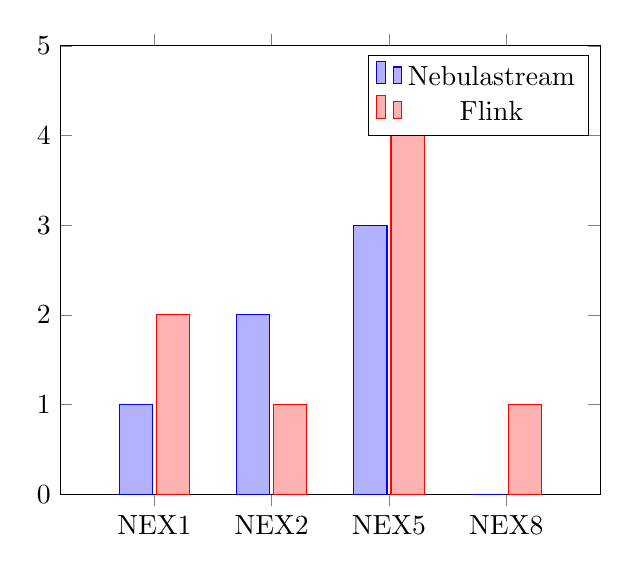
\begin{tikzpicture}

\begin{axis} [ybar = .05cm,
	bar width = 12pt,
	ymin = 0,
	ymax = 4,
	xtick = data,
        xticklabels={NEX1,NEX2,NEX5,NEX8},
	enlarge y limits = {value = .25, upper},
	enlarge x limits = {abs = .8}
]

\addplot coordinates {(0,1) (1,2) (2,3) (3,0)};
\addplot coordinates {(0,2) (1,1) (2,4) (3,1)};

\legend {Nebulastream, Flink};

\end{axis}

\end{tikzpicture}
    \caption{Caption}
    \label{fig:enter-label}
\end{figure}
\fi

\iffalse
\begin{figure}
    \centering
    %========== e2e latency of spes ========== begin
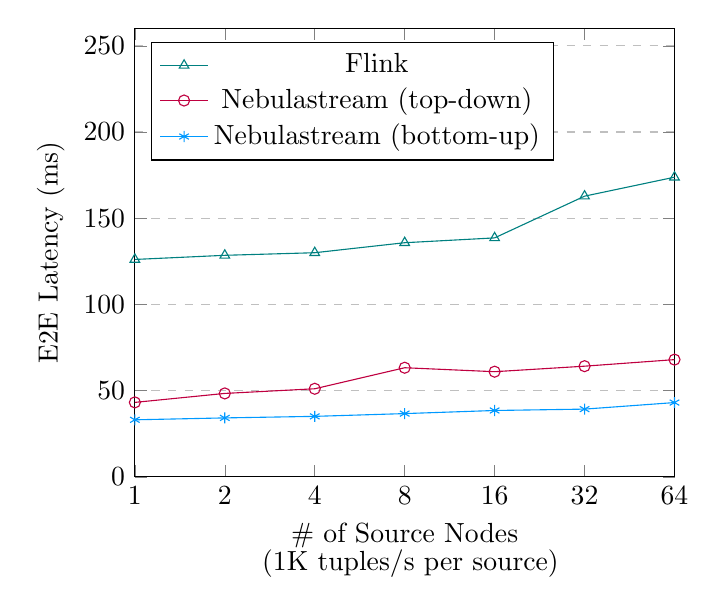
\begin{tikzpicture}
\begin{axis}[
    %title={End-to-end latency of the applications over scaling with $n$ nodes},
    xlabel={\# of Source Nodes},
    ylabel={E2E Latency (ms)},
    xmin=0, xmax=60,
    xticklabels={1,2,4,8,16,32,64},
    ymin=0, ymax=260,
    xtick={0,10,20,30,40,50,60},
    ytick={0,50,100,150,200,250},
    legend pos=north west,
    ymajorgrids=true,
    grid style=dashed,
]



\addplot[
    color=teal,
    mark=triangle,
    %dashed,
    ]
    coordinates {
    (0,126.1)(10,128.5)(20,130)(30,135.8)(40,138.6)(50,162.8)(60,173.8)
    };

\addplot[
    color=purple,
    mark=o,
    ]
    coordinates {
    (0,43.2)(10,48.4)(20,51.1)(30,63.3)(40,61)(50,64.2)(60,68)
    %(0,56.1)(10,59.5)(20,62)(30,64.8)(40,65.6)(50,66.8)(60,68)(70,77)
    };
    
\addplot[
    color=cyan,
    mark=asterisk,
    ]
    coordinates {
    (0,33.1)(10,34.2)(20,35.1)(30,36.7)(40,38.5)(50,39.3)(60,43.1)
    %(0,35.2)(10,35.5)(20,36)(30,37.8)(40,41.5)(50,42.4)(60,43.1)(70,44)
    };

\legend{Flink, Nebulastream (top-down), Nebulastream (bottom-up)}
    
\end{axis}
\node at (3.5,-1.1) {\textcolor{black}{(1K tuples/s per source)}};
\end{tikzpicture}


%========== e2e latency of spes ========== end
    \caption{End-to-end latency of SPEs over varying data source nodes. Nebulastream (top-down) (\textcolor{purple}{\st{{\raisebox{-1pt}{\large$\circ$}}}}) represents an enforced operator placement strategy at top nodes, where Nebulastream (bottom-up) (\textcolor{cyan}{\st{{\raisebox{-1pt}{\large$*$}}}}) applies optimization that places operators close to data sources.}
    \label{fig:enter-label}
\end{figure}
\fi

\iffalse
\begin{figure}
\centering
\begin{subfigure}{0.5\textwidth}
  \centering
  \includegraphics[width=0.7\linewidth]{figs/perf-measures-ph.png}
  \caption{Latency}
  \label{fig:sub11}
\end{subfigure}%
\hspace{-22mm}
\begin{subfigure}{0.5\textwidth}
  \centering
  \includegraphics[width=0.6\linewidth]{figs/topology-binary-tree.png}
  \caption{Topology}
  \label{fig:sub22}
\end{subfigure}
%\caption{Latency distribution of the SPSs along varying number of nodes with binary tree topology.}
\label{fig:test}

\vspace{1mm} % Adjust the vertical space between the rows if needed

\centering
\begin{subfigure}{0.5\textwidth}
  \centering
  \includegraphics[width=0.7\linewidth]{figs/perf-measures-ph.png}
  \caption{Latency}
  \label{fig:sub1}
\end{subfigure}%
\hspace{-22mm}
\begin{subfigure}{0.5\textwidth}
  \centering
  \includegraphics[width=0.6\linewidth]{figs/topology-2.png}
  \caption{Topology}
  \label{fig:sub2}
\end{subfigure}
\caption{Latency distribution of the SPSs along varying number of nodes with binary tree topology.}
\label{fig:testt}

\end{figure}
\fi


\subsection{Takeaways}

\iffalse
\begin{tikzpicture}
	\pgfplotstableread[col sep=comma]{data.csv}\csvdata
	% Boxplot groups columns, but we want rows
	\pgfplotstabletranspose\datatransposed{\csvdata} 
	\begin{axis}[
		boxplot/draw direction = y,
		%x axis line style = {opacity=0},
		axis x line* = bottom,
		axis y line = left,
		enlarge y limits,
		ymajorgrids,
		xtick = {1, 2, 3, 4},
		xticklabel style = {align=center, font=\small, rotate=0},
		xticklabels = {2, 3, 4, 5},
		%xtick style = {draw=none}, % Hide tick line
		ylabel = {E2E Latency},
            xlabel = {Topology Depth},
		ytick = {50, 100, 150, 200, 250}
	]
		\foreach \n in {1,...,4} {
			\addplot+[boxplot,
            fill, 
            draw=black, 
            mark=x, 
            mark options = {mark color=grey},
             %nodes near coords,  
             %nodes near coords align=right,
             ] table[y index=\n]
            {\datatransposed};
		}
	\end{axis}
\end{tikzpicture}
\fi

\iffalse
\begin{tikzpicture}
	\pgfplotstableread[col sep=comma]{data-numoftuples.csv}\csvdata
	% Boxplot groups columns, but we want rows
	\pgfplotstabletranspose\datatransposed{\csvdata} 
	\begin{axis}[
		boxplot/draw direction = y,
		%x axis line style = {opacity=0},
		axis x line* = bottom,
		axis y line = left,
		enlarge y limits,
		ymajorgrids,
		xtick = {1, 2, 3, 4},
		xticklabel style = {align=center, font=\small, rotate=60},
		xticklabels = {100, 500, 1000, 5000},
		%xtick style = {draw=none}, % Hide tick line
		ylabel = {E2E Latency},
            xlabel = {\# of Tuples per second},
		ytick = {50, 100, 150, 200, 250}
	]
		\foreach \n in {1,...,4} {
			\addplot+[boxplot,
            fill, 
            draw=black, 
            mark=x, 
            mark options = {mark color=grey},
             %nodes near coords,  
             %nodes near coords align=right,
             ] table[y index=\n]
            {\datatransposed};
		}
	\end{axis}
\end{tikzpicture}
\fi

\iffalse
\begin{tikzpicture}
	\pgfplotstableread[col sep=comma]{data-numoftuples-bottomtop.csv}\csvdata
	% Boxplot groups columns, but we want rows
	\pgfplotstabletranspose\datatransposed{\csvdata} 
	\begin{axis}[
		boxplot/draw direction = y,
		%x axis line style = {opacity=0},
		axis x line* = bottom,
		axis y line = left,
		enlarge y limits,
		ymajorgrids,
		xtick = {1, 3, 5, 7},
		xticklabel style = {align=center, font=\small, rotate=60},
		xticklabels = {100, 500, 1000, 5000},
		%xtick style = {draw=none}, % Hide tick line
		ylabel = {E2E Latency},
            xlabel = {\# of Tuples per second},
		ytick = {50, 100, 150, 200, 250}
	]
		\foreach \n in {1,...,8} {
			\addplot+[boxplot,
            fill, 
            draw=black, 
            mark=x, 
            mark options = {mark color=grey},
             %nodes near coords,  
             %nodes near coords align=right,
             ] table[y index=\n]
            {\datatransposed};
		}
	\end{axis}
\end{tikzpicture}
\fi

\pgfplotstableread[row sep=\\,col sep=&]{
    interval & carT & carD & carR \\
    25     & 1205 & 1043  & 0.2  \\ % 5x5=25
    100     & 1207 & 1047  & 4.9  \\ % 10x10=100
    10K    & 1385 & 1046 & 13.4 \\ % 100x100=10000
    1M   & 1389 & 1058 & 22.2 \\ % 1000x1000=1m
    25M   & 1449 & 0 & 27.0 \\ %5kx5k=25m
    100M      & 1524  & 0 & 28.6 \\ %10kx10k=100m
    }\mydata

\iffalse
\begin{tikzpicture}
    \begin{axis}[
            ybar,
            bar width=.5cm,
            width=1.1\textwidth,
            height=.6\textwidth,
            legend style={at={(0.7,1.2)},
                anchor=north,legend columns=-1},
            symbolic x coords={25,100,10K,1M,25M,100M},
            xtick=data,
            nodes near coords,
            every node near coord/.append style={font=\footnotesize, rotate=90, anchor=west},
            nodes near coords align={vertical},
            ymin=0,
            ymax=2000,
            ylabel={E2E Latency (ms)},
            xlabel={\# of Produced Tuples},
        ]
        \addplot[draw=blue0, semithick, pattern = north west lines, fill=blue0] table[x=interval,y=carT]{\mydata};
        \addplot[draw=blue1, thick, pattern = north west lines, pattern color=blue1] table[x=interval,y=carD]{\mydata};
        %\addplot table[x=interval,y=carR]{\mydata};
        \legend{Bottom-Up, Top-Down, Energy}
    \end{axis}
    \node [rotate=90] at (9.1,2.2) {\textcolor{blue1}{Failure}};
    \node [rotate=90] at (11.1,2.2) {\textcolor{blue1}{Failure}};
    %\node at (9,-1.0) {\textcolor{darkgray}{Backpressure}};
    %\draw [dashed, darkgray] (8,-0.8) -- (8,6);
\end{tikzpicture}
\fi



\begin{filecontents*}{data-numoftuples-bottomtop.csv}
102.6, 103.1, 203.1, 102.7, 103.1, 41.4, 202.3, 105.5, 104.4, 106.6, 104.9, 104.6 %100b
106.7, 105.8, 107.7, 104.2, 104.3, 106.5, 204.7, 105.9, 105.3, 104.1, 105.0, 107.6 %100t
120.2, 125.9, 121.3, 123.8, 221.5, 121.7, 43.4, 123.6, 121.8, 111.7, 123.5, 121.1 %500b
123.3, 121.4, 120.0, 123.1, 120.0, 220.5, 121.9, 122.7, 120.6, 120.6, 119.1, 124.2 %500t
127.3, 126.2, 128.4, 124.6, 148.3, 149.2, 225.1, 135, 51, 132, 115, 135 %1000b
128.5, 132.3, 132.1, 225.2, 128.8, 133.4, 125.7, 123.1, 127.6, 125.6, 222.3, 138.4 %1000t
152.3, 193.2, 199.7, 210.3, 183.7, 209.2, 150.5, 216.5, 142.4, 140.1, 116.1, 148.8 %5000b
145.2, 201.3, 157.4, 195.6, 191.3, 184.4, 133.3, 148.4, 176.6, 184.0, 199.9, 206.6 %5000t
\end{filecontents*}

\pgfplotstableread[row sep=\\,col sep=&]{
    interval & carT & carD & carR \\
    100     & 43 & 46  & 0.2  \\ % 5x5=25
    500     & 60 & 65 & 4.9  \\ % 10x10=100
    1K    & 67 & 68 & 13.4 \\ % 100x100=10000
    5K   & 92 & 110 & 22.2 \\ % 1000x1000=1m
    100K   & 344 & 0 & 27.0 \\ %5kx5k=25m
    1M      & 589  & 0 & 28.6 \\ %10kx10k=100m
    }\mydatanexmarkqonenumoftuples

\iffalse
\begin{tikzpicture}
    \begin{axis}[
            ybar,
            bar width=.5cm,
            width=1.1\textwidth,
            height=.6\textwidth,
            legend style={at={(0.7,1.2)},
                anchor=north,legend columns=-1},
            symbolic x coords={100,500,1K,5K,100K,1M},
            xtick=data,
            nodes near coords,
            every node near coord/.append style={font=\footnotesize, rotate=90, anchor=west},
            nodes near coords align={vertical},
            ymin=0,
            ymax=700,
            ylabel={E2E Latency (ms)},
            xlabel={\# of Input Tuples per Second},
        ]
        \addplot[draw=blue0, semithick, pattern = north west lines, fill=blue0] table[x=interval,y=carT]{\mydatanexmarkqonenumoftuples};
        \addplot[draw=blue1, thick, pattern = north west lines, pattern color=blue1] table[x=interval,y=carD]{\mydatanexmarkqonenumoftuples};
        %\addplot table[x=interval,y=carR]{\mydata};
        \legend{Bottom-Up, Top-Down, Energy}
    \end{axis}
    \node [rotate=90] at (9.1,1.2) {\textcolor{blue1}{Failure}};
    \node [rotate=90] at (11.1,1.2) {\textcolor{blue1}{Failure}};
    %\node at (9,-1.0) {\textcolor{darkgray}{Backpressure}};
    %\draw [dashed, darkgray] (8,-0.8) -- (8,6);
\end{tikzpicture}
\fi





%=========================================================

\pgfplotstableread[row sep=\\,col sep=&]{
    interval & carT & carD & carR \\
    25     & 1703 & 1241  & 0.2  \\ % 5x5=25
    100     & 1723 & 1278  & 4.9  \\ % 10x10=100
    10K    & 2125 & 1855 & 13.4 \\ % 100x100=10000
    1M   & 4023 & 2253 & 22.2 \\ % 1000x1000=1m
    4M   & 6778 & 2981 & 27.0 \\ %2kx2k=4m
    25M      & 9776  & 0 & 28.6 \\ %5kx5k=25m
    }\mydataa

\iffalse
\begin{tikzpicture}
    \begin{axis}[
            ybar,
            bar width=.5cm,
            width=1.1\textwidth,
            height=.6\textwidth,
            legend style={at={(0.5,1.2)},
                anchor=north,legend columns=-1},
            symbolic x coords={25,100,10K,1M,4M,25M},
            xtick=data,
            nodes near coords,
            every node near coord/.append style={font=\footnotesize, rotate=90, anchor=west},
            nodes near coords align={vertical},
            ymin=0,
            ymax=10500,
            ylabel={E2E Latency (ms)},
            xlabel={\# of Downstream Tuples},
        ]
        \addplot table[x=interval,y=carT, draw=blue]{\mydataa};
        \addplot table[x=interval,y=carD, draw=red]{\mydataa};
        %\addplot table[x=interval,y=carR]{\mydata};
        \legend{Bottom-Up, Top-Down, Energy}
    \end{axis}
    \node [rotate=90] at (11.1,1.2) {\textcolor{red}{Failure}};
    \node at (13,2.8) {\textcolor{darkgray}{Backpressure}};
    \draw [dashed, darkgray] (0,2.6) -- (13,2.6);
\end{tikzpicture}
\fi

%========== execution time distr. of kernels ========== begin
\iffalse
\begin{figure*}[h]
  \centering
  
  \pgfplotsset{every tick label/.append style={font=\tiny}}

\pgfplotstableread{ % data 
Label       Network   Brokers  Processing    other
Cora        26.2    8      8.1            45
CiteSeer    22.2    7      5.3            45
Pubmed      24.7    6       12.6          45
Reddit      28.2    7       8             45
LiveJournal 25      8       7             45
    }\datanesbottomup

\pgfplotstableread{ % data 
Label       Network   Brokers  Processing    other
Cora        26.2    8      8.1            45
CiteSeer    22.2    7      5.3            45
Pubmed      24.7    6       12.6          45
Reddit      28.2    7       8             45
LiveJournal 25      8       7             45
    }\datanestopdown
  
\pgfplotstableread{ % data 
Label       Network   Brokers  Processing    other
Cora        26.2    8      8.1            45
CiteSeer    22.2    7      5.3            45
Pubmed      24.7    6       12.6          45
Reddit      28.2    7       8             45
LiveJournal 25      8       7             45
    }\datapyggcn
    
\pgfplotstableread{ % data 
Label       Network   Brokers  Processing    other
Cora        26.2     8     29.3           23
CiteSeer    22.2     7     23.5           23
Pubmed      24.7     6     33.9           23
Reddit      28.2     7       34           23
LiveJournal 25       8       36           23
    }\datapyggin
    
\pgfplotstableread{ % data 
Label       Network   Brokers  Processing    other
Cora        26.2    8     39.7           13
CiteSeer    22.2    7     32.5           13
Pubmed      24.7    6     39.7           13
Reddit      28.2     7       35             13
LiveJournal 25       8       34             13
    }\datapygsag
    
    
    
\pgfplotstableread{ % data 
Label       (De-)Serialization    Network    other
Cora        69.8    6.6      23.6
CiteSeer    70.2    6.9      22.9
Pubmed      73.0    7.2      19.8
Reddit      78      8        14
LiveJournal 85      10       5
    }\datadglgcn
    
\pgfplotstableread{ % data 
Label       (De-)Serialization    Network    other
Cora        50.6    6.1      43.3
CiteSeer    53.4    5.7      40.9
Pubmed      60.6    5.4      34
Reddit      66      4        30
LiveJournal 68      4        28
    }\datadglgin
    
\pgfplotstableread{ % data 
Label       (De-)Serialization    Network    other
Cora        48.2    5.1      46.7
CiteSeer    52.2    5.0      42.8
Pubmed      53.5    5.2      41.3
Reddit      78      8        14
LiveJournal 85      10       5
    }\datadglsag
    
    

\pgfplotstableread{ % data 
Label       Network   Brokers  Processing    other
Cora        70.2    10.6     9.2            10
CiteSeer    62.1    9.1      13.8           15
Pubmed      39.2    27.1     21.7           12
Reddit      37      30       24             9
LiveJournal 35      34       22             9
    }\datagsuitempgcn
    
\pgfplotstableread{ % data 
Label       Network   Brokers  Processing    other
Cora        2.2     37.2     57.3           3.3
CiteSeer    2.8     34.1     56.2           6.9
Pubmed      3.6     36.8     55.4           4.2
Reddit      5       34       52             9
LiveJournal 7       33       47             13
    }\datagsuitempgin
    
\pgfplotstableread{ % data 
Label       Network   Brokers  Processing    other
Cora        8.1     36.0     39.7           16.2
CiteSeer    15.8    31.7     32.5           20
Pubmed      7.6     39.1     39.7           13.6
Reddit      6       40       35             19
LiveJournal 5       44       33             18
    }\datagsuitempsag
    
    

\pgfplotstableread{ % data 
Label       (De-)Serialization    Network    other
Cora        77.8    8.6      13.6
CiteSeer    80.2    6.9      12.9
Pubmed      82.0    8.2      9.8
Reddit      85      8        7
LiveJournal 86      7        7
    }\datagsuitespmmgcn
    
\pgfplotstableread{ % data 
Label       (De-)Serialization    Network    other
Cora        63.6    10.1     26.3
CiteSeer    63.4    8.7      27.9
Pubmed      71.6    8.4      20
Reddit      74      6        20
LiveJournal 77      4        19
    }\datagsuitespmmgin
    
\pgfplotstableread{ % data 
Label       (De-)Serialization    Network    other
Cora        62.2    8.1      29.7
CiteSeer    65.2    9.0      26.8
Pubmed      63.5    10.2     26.3
Reddit      65      12       23
LiveJournal 68      15       17
    }\datagsuitespmmsag
    
\pgfplotstableread{ % data 
Label       Network   Brokers  Processing   (De-)Serialization  other
Cora        0       0        0             0     0
}\datalegend


    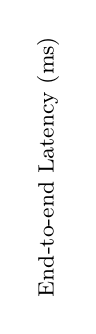
\begin{tikzpicture}
        \node[align=center] at (0,2) {\rotatebox{90}{\footnotesize{End-to-end Latency (ms)}}};
    \end{tikzpicture}
    \begin{tikzpicture}[framed]

    \node at (3,4.5) {\footnotesize Stream Processing System};
    \node at (3,-0.8) {\footnotesize TPC-H Queries};

    \begin{axis}[
    width=3.5cm,
    height=5cm,
    title={Our System},
    title style = {font=\footnotesize},
    ybar stacked,   % Stacked horizontal bars
    bar width = 0.35cm,
    ymin=0,         % Start x axis at 0
    xtick=data,     % Use as many tick labels as y coordinates
    legend style={at={(axis cs:105,0)},anchor=south west, font=\footnotesize},
    %xlabel={Distribution of Stall Reasons (\%)},
    ytick={0,25,50,75,100},
    xticklabels = {T1,T3,T7,T8,T10},  % Get the labels from the Label column of the \datatable
    xticklabel style={rotate=90}
    ]
    \addplot [draw = blue0,
    semithick,
    pattern = north west lines,
    fill = blue0] table [y=Network, meta=Label,x expr=\coordindex] {\datapyggcn};   % "First" column against the data index
    \addplot [draw = blue2,
    semithick,
    pattern = crosshatch,
    fill = blue2] table [y=Brokers, meta=Label,x expr=\coordindex] {\datapyggcn};
    \addplot [draw = blue1,
    semithick,
    pattern = north west lines,
    pattern color = blue1] table [y=Processing, meta=Label,x expr=\coordindex] {\datapyggcn};
    \addplot [draw = white,
    semithick,
    pattern = grid,
    fill = white] table [y=other, meta=Label,x expr=\coordindex] {\datapyggcn};
    \end{axis}
    
    \begin{axis}[
    width=3.5cm,
    height=5cm,
    title={Flink},
    title style = {font=\footnotesize},
    xshift=2.1cm,
    ybar stacked,   % Stacked horizontal bars
    bar width = 0.35cm,
    ymin=0,         % Start x axis at 0
    xtick=data,     % Use as many tick labels as y coordinates
    legend style={at={(axis cs:8,-7.5)},anchor=south west},
    %xlabel={Distribution of Stall Reasons (\%)},
    %ytick={0,25,50,75,100},
    yticklabels={,,},
    %yticklabels from table={\testdata}{Label},  % Get the labels from the Label column of the \datatable
    xticklabels = {CR,CS,PB,RD,LJ},
    xticklabel style={rotate=90}
    ]
    \addplot [draw = blue0,
    semithick,
    pattern = north west lines,
    fill = blue0] table [y=Network, meta=Label,x expr=\coordindex] {\datapyggin};   % "First" column against the data index
    \addplot [draw = blue2,
    semithick,
    pattern = crosshatch,
    fill = blue2] table [y=Brokers, meta=Label,x expr=\coordindex] {\datapyggin};
    \addplot [draw = blue1,
    semithick,
    pattern = north west lines,
    pattern color = blue1] table [y=Processing, meta=Label,x expr=\coordindex] {\datapyggin};
    \addplot [draw = blue4,
    semithick,
    pattern = grid,
    fill = blue4] table [y=other, meta=Label,x expr=\coordindex] {\datapyggin};
    %\legend{Network,Brokers,Processing,other}
    \end{axis}
    
    \begin{axis}[
    width=3.5cm,
    height=5cm,
    xshift=4.2cm,
    title={Spark Streaming},
    title style = {font=\footnotesize},
    ybar stacked,   % Stacked horizontal bars
    bar width = 0.35cm,
    ymin=0,         % Start x axis at 0
    xtick=data,     % Use as many tick labels as y coordinates
    legend style={at={(axis cs:55,0)},anchor=south west, font=\footnotesize},
    %xlabel={Distribution of Stall Reasons (\%)},
    yticklabels={,,},
    xticklabels = {CR,CS,PB,RD,LJ},  % Get the labels from the Label column of the \datatable
    xticklabel style={rotate=90}
    ]
    \addplot [draw = blue0,
    semithick,
    pattern = north west lines,
    fill = blue0] table [y=Network, meta=Label,x expr=\coordindex] {\datapygsag};   % "First" column against the data index
    \addplot [draw = blue2,
    semithick,
    pattern = crosshatch,
    fill = blue2] table [y=Brokers, meta=Label,x expr=\coordindex] {\datapygsag};
    \addplot [draw = blue1,
    semithick,
    pattern = north west lines,
    pattern color = blue1] table [y=Processing, meta=Label,x expr=\coordindex] {\datapygsag};
    \addplot [draw = blue4,
    semithick,
    pattern = grid,
    fill = blue4] table [y=other, meta=Label,x expr=\coordindex] {\datapygsag};
    \end{axis}
    
    
    \end{tikzpicture}
    
    
%    \begin{axis}[
%    width=2.5cm,
%    height=3.3cm,
%    xshift=2.2cm,
%    title={SAG},
%    title style = {font=\footnotesize},
%    ybar stacked,   % Stacked horizontal bars
%    bar width = 0.14cm,
%    ymin=0,         % Start x axis at 0
%    xtick=data,     % Use as many tick labels as y coordinates
%    legend style={at={(axis cs:55,0)},anchor=south west, font=\footnotesize},
%    %xlabel={Distribution of Stall Reasons (\%)},
%    yticklabels={,,},
%    xticklabels = {CR,CS,PB,RD,LJ},  % Get the labels from the Label column of the \datatable
%    xticklabel style={rotate=90}
%    ]
%     \addplot [draw = blue3,
%    semithick,
%    pattern = crosshatch,
%    pattern color=blue3] table [y=(De-)Serialization, meta=Label,x expr=\coordindex] {\datagsuitespmmsag};   % "First" column against the data index
%    \addplot [draw = blue0,
%    semithick,
%    pattern = north west lines,
%    fill = blue0] table [y=Network, meta=Label,x expr=\coordindex] {\datagsuitespmmsag};
%    \addplot [draw = blue4,
%    semithick,
%    pattern = grid,
%    fill = blue4] table [y=other, meta=Label,x expr=\coordindex] {\datagsuitespmmsag};
%    \end{axis}
    
    
    \begin{tikzpicture}

    \begin{axis}[
    width=3cm,
    height=1.7cm,
    %title={GCN},
    title style = {font=\footnotesize},
    axis line style={draw=none},
    ticks = none,
    ybar stacked,   % Stacked horizontal bars
    %bar width = 0.25cm,
    ymin=0,         % Start x axis at 0
    %xtick=data,     % Use as many tick labels as y coordinates
    legend style={at={(axis cs:-7,0)},anchor=south west, font=\footnotesize, /tikz/every even column/.append style={column sep=0.2cm}},
    legend columns=5,
    %xlabel={Distribution of Stall Reasons (\%)},
    %ytick={0,25,50,75,100},
    %xticklabels = {CR,CS,PB},  % Get the labels from the Label column of the \datatable
    %xticklabel style={rotate=75}
    ]
    \addplot [draw = blue0,
    semithick,
    pattern = north west lines,
    fill = blue0] table [y=Network, meta=Label,x expr=\coordindex] {\datalegend};   % "First" column against the data index
    \addplot [draw = blue2,
    semithick,
    pattern = crosshatch,
    fill = blue2] table [y=Brokers, meta=Label,x expr=\coordindex] {\datalegend};
    \addplot [draw = blue1,
    semithick,
    pattern = north west lines,
    pattern color = blue1] table [y=Processing, meta=Label,x expr=\coordindex] {\datalegend};
    \addplot [draw = blue3,
    semithick,
    pattern = crosshatch,
    pattern color=blue3] table [y=(De-)Serialization, meta=Label,x expr=\coordindex] {\datalegend};
    \addplot [draw = blue4,
    semithick,
    pattern = grid,
    fill = blue4] table [y=other, meta=Label,x expr=\coordindex] {\datalegend};
    \legend{Network,Brokers,Processing,(De-)Serialization,other}
    \end{axis}
    
    
    
    \end{tikzpicture}

    \caption{End-to-end latency distribution of the applications over different stream processing systems.}
    \label{fig:exec-time-dist-kernelss}

\end{figure*}
\fi
%========== execution time distr. of kernels ========== end


%========== execution time distr. of kernels ========== begin
\iffalse
\begin{figure*}[h]
  \centering
  
  \pgfplotsset{every tick label/.append style={font=\tiny}}
  
  
\pgfplotstableread{ % data 
Label       Network   Brokers  Processing    other
Cora        26.2    8      8.1            45
CiteSeer    22.2    7      5.3            45
Pubmed      24.7    6       12.6          45
Reddit      28.2    7       8             45
LiveJournal 25      8       7             45
    }\datapyggcn
    
\pgfplotstableread{ % data 
Label       Network   Brokers  Processing    other
Cora        26.2     8     29.3           23
CiteSeer    22.2     7     23.5           23
Pubmed      24.7     6     33.9           23
Reddit      28.2     7       34           23
LiveJournal 25       8       36           23
    }\datapyggin
    
\pgfplotstableread{ % data 
Label       Network   Brokers  Processing    other
Cora        26.2    8     39.7           13
CiteSeer    22.2    7     32.5           13
Pubmed      24.7    6     39.7           13
Reddit      28.2     7       35             13
LiveJournal 25       8       34             13
    }\datapygsag
    
    
    
\pgfplotstableread{ % data 
Label       (De-)Serialization    Network    other
Cora        69.8    6.6      23.6
CiteSeer    70.2    6.9      22.9
Pubmed      73.0    7.2      19.8
Reddit      78      8        14
LiveJournal 85      10       5
    }\datadglgcn
    
\pgfplotstableread{ % data 
Label       (De-)Serialization    Network    other
Cora        50.6    6.1      43.3
CiteSeer    53.4    5.7      40.9
Pubmed      60.6    5.4      34
Reddit      66      4        30
LiveJournal 68      4        28
    }\datadglgin
    
\pgfplotstableread{ % data 
Label       (De-)Serialization    Network    other
Cora        48.2    5.1      46.7
CiteSeer    52.2    5.0      42.8
Pubmed      53.5    5.2      41.3
Reddit      78      8        14
LiveJournal 85      10       5
    }\datadglsag
    
    

\pgfplotstableread{ % data 
Label       Network   Brokers  Processing    other
Cora        70.2    10.6     9.2            10
CiteSeer    62.1    9.1      13.8           15
Pubmed      39.2    27.1     21.7           12
Reddit      37      30       24             9
LiveJournal 35      34       22             9
    }\datagsuitempgcn
    
\pgfplotstableread{ % data 
Label       Network   Brokers  Processing    other
Cora        2.2     37.2     57.3           3.3
CiteSeer    2.8     34.1     56.2           6.9
Pubmed      3.6     36.8     55.4           4.2
Reddit      5       34       52             9
LiveJournal 7       33       47             13
    }\datagsuitempgin
    
\pgfplotstableread{ % data 
Label       Network   Brokers  Processing    other
Cora        8.1     36.0     39.7           16.2
CiteSeer    15.8    31.7     32.5           20
Pubmed      7.6     39.1     39.7           13.6
Reddit      6       40       35             19
LiveJournal 5       44       33             18
    }\datagsuitempsag
    
    

\pgfplotstableread{ % data 
Label       (De-)Serialization    Network    other
Cora        77.8    8.6      13.6
CiteSeer    80.2    6.9      12.9
Pubmed      82.0    8.2      9.8
Reddit      85      8        7
LiveJournal 86      7        7
    }\datagsuitespmmgcn
    
\pgfplotstableread{ % data 
Label       (De-)Serialization    Network    other
Cora        63.6    10.1     26.3
CiteSeer    63.4    8.7      27.9
Pubmed      71.6    8.4      20
Reddit      74      6        20
LiveJournal 77      4        19
    }\datagsuitespmmgin
    
\pgfplotstableread{ % data 
Label       (De-)Serialization    Network    other
Cora        62.2    8.1      29.7
CiteSeer    65.2    9.0      26.8
Pubmed      63.5    10.2     26.3
Reddit      65      12       23
LiveJournal 68      15       17
    }\datagsuitespmmsag
    
\pgfplotstableread{ % data 
Label       Network   Brokers  Processing   (De-)Serialization  other
Cora        0       0        0             0     0
}\datalegend


    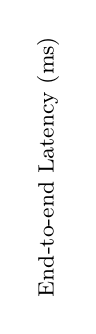
\begin{tikzpicture}
        \node[align=center] at (0,2) {\rotatebox{90}{\footnotesize{End-to-end Latency (ms)}}};
    \end{tikzpicture}
    \begin{tikzpicture}[framed]

    \node at (3,4.5) {\footnotesize Stream Processing System};
    \node at (3,-0.8) {\footnotesize TPC-H Queries};

    \begin{axis}[
    width=3.5cm,
    height=5cm,
    title={Our System},
    title style = {font=\footnotesize},
    ybar stacked,   % Stacked horizontal bars
    bar width = 0.35cm,
    ymin=0,         % Start x axis at 0
    xtick=data,     % Use as many tick labels as y coordinates
    legend style={at={(axis cs:105,0)},anchor=south west, font=\footnotesize},
    %xlabel={Distribution of Stall Reasons (\%)},
    ytick={0,25,50,75,100},
    xticklabels = {T1,T3,T7,T8,T10},  % Get the labels from the Label column of the \datatable
    xticklabel style={rotate=90}
    ]
    \addplot [draw = blue0,
    semithick,
    pattern = north west lines,
    fill = blue0] table [y=Network, meta=Label,x expr=\coordindex] {\datapyggcn};   % "First" column against the data index
    \addplot [draw = blue2,
    semithick,
    pattern = crosshatch,
    fill = blue2] table [y=Brokers, meta=Label,x expr=\coordindex] {\datapyggcn};
    \addplot [draw = blue1,
    semithick,
    pattern = north west lines,
    pattern color = blue1] table [y=Processing, meta=Label,x expr=\coordindex] {\datapyggcn};
    \addplot [draw = white,
    semithick,
    pattern = grid,
    fill = white] table [y=other, meta=Label,x expr=\coordindex] {\datapyggcn};
    \end{axis}
    
    \begin{axis}[
    width=3.5cm,
    height=5cm,
    title={Flink},
    title style = {font=\footnotesize},
    xshift=2.1cm,
    ybar stacked,   % Stacked horizontal bars
    bar width = 0.35cm,
    ymin=0,         % Start x axis at 0
    xtick=data,     % Use as many tick labels as y coordinates
    legend style={at={(axis cs:8,-7.5)},anchor=south west},
    %xlabel={Distribution of Stall Reasons (\%)},
    %ytick={0,25,50,75,100},
    yticklabels={,,},
    %yticklabels from table={\testdata}{Label},  % Get the labels from the Label column of the \datatable
    xticklabels = {CR,CS,PB,RD,LJ},
    xticklabel style={rotate=90}
    ]
    \addplot [draw = blue0,
    semithick,
    pattern = north west lines,
    fill = blue0] table [y=Network, meta=Label,x expr=\coordindex] {\datapyggin};   % "First" column against the data index
    \addplot [draw = blue2,
    semithick,
    pattern = crosshatch,
    fill = blue2] table [y=Brokers, meta=Label,x expr=\coordindex] {\datapyggin};
    \addplot [draw = blue1,
    semithick,
    pattern = north west lines,
    pattern color = blue1] table [y=Processing, meta=Label,x expr=\coordindex] {\datapyggin};
    \addplot [draw = blue4,
    semithick,
    pattern = grid,
    fill = blue4] table [y=other, meta=Label,x expr=\coordindex] {\datapyggin};
    %\legend{Network,Brokers,Processing,other}
    \end{axis}
    
    \begin{axis}[
    width=3.5cm,
    height=5cm,
    xshift=4.2cm,
    title={Spark Streaming},
    title style = {font=\footnotesize},
    ybar stacked,   % Stacked horizontal bars
    bar width = 0.35cm,
    ymin=0,         % Start x axis at 0
    xtick=data,     % Use as many tick labels as y coordinates
    legend style={at={(axis cs:55,0)},anchor=south west, font=\footnotesize},
    %xlabel={Distribution of Stall Reasons (\%)},
    yticklabels={,,},
    xticklabels = {CR,CS,PB,RD,LJ},  % Get the labels from the Label column of the \datatable
    xticklabel style={rotate=90}
    ]
    \addplot [draw = blue0,
    semithick,
    pattern = north west lines,
    fill = blue0] table [y=Network, meta=Label,x expr=\coordindex] {\datapygsag};   % "First" column against the data index
    \addplot [draw = blue2,
    semithick,
    pattern = crosshatch,
    fill = blue2] table [y=Brokers, meta=Label,x expr=\coordindex] {\datapygsag};
    \addplot [draw = blue1,
    semithick,
    pattern = north west lines,
    pattern color = blue1] table [y=Processing, meta=Label,x expr=\coordindex] {\datapygsag};
    \addplot [draw = blue4,
    semithick,
    pattern = grid,
    fill = blue4] table [y=other, meta=Label,x expr=\coordindex] {\datapygsag};
    \end{axis}
    
    
    \end{tikzpicture}
    
    
%    \begin{axis}[
%    width=2.5cm,
%    height=3.3cm,
%    xshift=2.2cm,
%    title={SAG},
%    title style = {font=\footnotesize},
%    ybar stacked,   % Stacked horizontal bars
%    bar width = 0.14cm,
%    ymin=0,         % Start x axis at 0
%    xtick=data,     % Use as many tick labels as y coordinates
%    legend style={at={(axis cs:55,0)},anchor=south west, font=\footnotesize},
%    %xlabel={Distribution of Stall Reasons (\%)},
%    yticklabels={,,},
%    xticklabels = {CR,CS,PB,RD,LJ},  % Get the labels from the Label column of the \datatable
%    xticklabel style={rotate=90}
%    ]
%     \addplot [draw = blue3,
%    semithick,
%    pattern = crosshatch,
%    pattern color=blue3] table [y=(De-)Serialization, meta=Label,x expr=\coordindex] {\datagsuitespmmsag};   % "First" column against the data index
%    \addplot [draw = blue0,
%    semithick,
%    pattern = north west lines,
%    fill = blue0] table [y=Network, meta=Label,x expr=\coordindex] {\datagsuitespmmsag};
%    \addplot [draw = blue4,
%    semithick,
%    pattern = grid,
%    fill = blue4] table [y=other, meta=Label,x expr=\coordindex] {\datagsuitespmmsag};
%    \end{axis}
    
    
    \begin{tikzpicture}

    \begin{axis}[
    width=3cm,
    height=1.7cm,
    %title={GCN},
    title style = {font=\footnotesize},
    axis line style={draw=none},
    ticks = none,
    ybar stacked,   % Stacked horizontal bars
    %bar width = 0.25cm,
    ymin=0,         % Start x axis at 0
    %xtick=data,     % Use as many tick labels as y coordinates
    legend style={at={(axis cs:-7,0)},anchor=south west, font=\footnotesize, /tikz/every even column/.append style={column sep=0.2cm}},
    legend columns=5,
    %xlabel={Distribution of Stall Reasons (\%)},
    %ytick={0,25,50,75,100},
    %xticklabels = {CR,CS,PB},  % Get the labels from the Label column of the \datatable
    %xticklabel style={rotate=75}
    ]
    \addplot [draw = blue0,
    semithick,
    pattern = north west lines,
    fill = blue0] table [y=Network, meta=Label,x expr=\coordindex] {\datalegend};   % "First" column against the data index
    \addplot [draw = blue2,
    semithick,
    pattern = crosshatch,
    fill = blue2] table [y=Brokers, meta=Label,x expr=\coordindex] {\datalegend};
    \addplot [draw = blue1,
    semithick,
    pattern = north west lines,
    pattern color = blue1] table [y=Processing, meta=Label,x expr=\coordindex] {\datalegend};
    \addplot [draw = blue3,
    semithick,
    pattern = crosshatch,
    pattern color=blue3] table [y=(De-)Serialization, meta=Label,x expr=\coordindex] {\datalegend};
    \addplot [draw = blue4,
    semithick,
    pattern = grid,
    fill = blue4] table [y=other, meta=Label,x expr=\coordindex] {\datalegend};
    \legend{Network,Brokers,Processing,(De-)Serialization,other}
    \end{axis}
    
    
    
    \end{tikzpicture}

    \caption{End-to-end latency distribution of the applications over different stream processing systems.}
    \label{fig:exec-time-dist-kernels}

\end{figure*}
\fi
%========== execution time distr. of kernels ========== end

%========== e2e latency of spes ========== begin
\iffalse
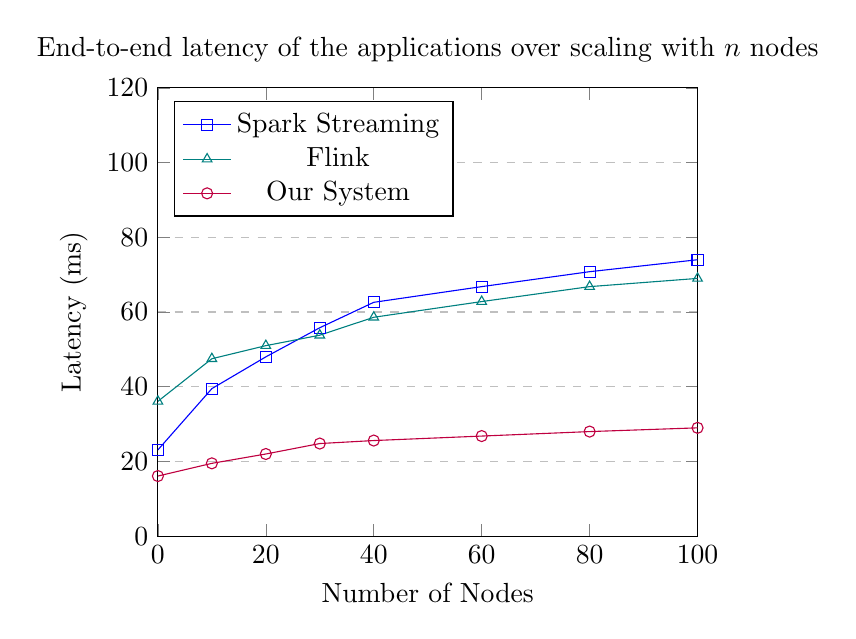
\begin{tikzpicture}
\begin{axis}[
    title={End-to-end latency of the applications over scaling with $n$ nodes},
    xlabel={Number of Nodes},
    ylabel={Latency (ms)},
    xmin=0, xmax=100,
    ymin=0, ymax=120,
    xtick={0,20,40,60,80,100},
    ytick={0,20,40,60,80,100,120},
    legend pos=north west,
    ymajorgrids=true,
    grid style=dashed,
]

\addplot[
    color=blue,
    mark=square,
    ]
    coordinates {
    (0,23.1)(10,39.5)(20,48)(30,55.8)(40,62.6)(60,66.8)(80,70.8)(100,74)
    };

\addplot[
    color=teal,
    mark=triangle,
    ]
    coordinates {
    (0,36.1)(10,47.5)(20,51)(30,53.8)(40,58.6)(60,62.8)(80,66.8)(100,69)
    };

\addplot[
    color=purple,
    mark=o,
    ]
    coordinates {
    (0,16.1)(10,19.5)(20,22)(30,24.8)(40,25.6)(60,26.8)(80,28)(100,29)
    };
    \legend{Spark Streaming, Flink, Our System}
    
\end{axis}
\end{tikzpicture}
\fi
%========== e2e latency of spes ========== end




\section{Related Work}

Attempt on assessing the performance of SPSs has been a thing for more than two decades now, initiated with Linear Road Benchmark\cite{linearroad04}.


Linear Road Benchmark'04

NEXMark'08

Yahoo Streaming Benchmark'16

RIoTBench'17

Karimov et al.'18

Liu et al.'19

Nasiri et al.'19

Vikash et al.'20

OSPBench'20

Theodolite'21

Theodorakis'22

PDSPBench'24

\section{Limitations and Future Work}

\section{Conclusion}








\subsection{A Subsection Sample}
Please note that the first paragraph of a section or subsection is
not indented. The first paragraph that follows a table, figure,
equation etc. does not need an indent, either.

Subsequent paragraphs, however, are indented.

\subsubsection{Sample Heading (Third Level)} Only two levels of
headings should be numbered. Lower level headings remain unnumbered;
they are formatted as run-in headings.

\paragraph{Sample Heading (Fourth Level)}
The contribution should contain no more than four levels of
headings. Table~\ref{tab1} gives a summary of all heading levels.

\begin{table}
\caption{Table captions should be placed above the
tables.}\label{tab1}
\begin{tabular}{|l|l|l|}
\hline
Heading level &  Example & Font size and style\\
\hline
Title (centered) &  {\Large\bfseries Lecture Notes} & 14 point, bold\\
1st-level heading &  {\large\bfseries 1 Introduction} & 12 point, bold\\
2nd-level heading & {\bfseries 2.1 Printing Area} & 10 point, bold\\
3rd-level heading & {\bfseries Run-in Heading in Bold.} Text follows & 10 point, bold\\
4th-level heading & {\itshape Lowest Level Heading.} Text follows & 10 point, italic\\
\hline
\end{tabular}
\end{table}


\noindent Displayed equations are centered and set on a separate
line.




Please try to avoid rasterized images for line-art diagrams and
schemas. Whenever possible, use vector graphics instead (see
Fig.~\ref{fig1}).

\begin{figure}
\includegraphics[width=\textwidth]{fig1.eps}
\caption{A figure caption is always placed below the illustration.
Please note that short captions are centered, while long ones are
justified by the macro package automatically.} \label{fig1}
\end{figure}

\begin{theorem}
This is a sample theorem. The run-in heading is set in bold, while
the following text appears in italics. Definitions, lemmas,
propositions, and corollaries are styled the same way.
\end{theorem}
%
% the environments 'definition', 'lemma', 'proposition', 'corollary',
% 'remark', and 'example' are defined in the LLNCS documentclass as well.
%
\begin{proof}
Proofs, examples, and remarks have the initial word in italics,
while the following text appears in normal font.
\end{proof}
For citations of references, we prefer the use of square brackets
and consecutive numbers. Citations using labels or the author/year
convention are also acceptable. The following bibliography provides
a sample reference list with entries for journal
articles~\cite{ref_article1}, an LNCS chapter~\cite{ref_lncs1}, a
book~\cite{ref_book1}, proceedings without editors~\cite{ref_proc1},
and a homepage~\cite{ref_url1}. Multiple citations are grouped
\cite{ref_article1,ref_lncs1,ref_book1},
\cite{ref_article1,ref_book1,ref_proc1,ref_url1}.

\begin{credits}
\subsubsection{\ackname} A bold run-in heading in small font size at the end of the paper is
used for general acknowledgments, for example: This study was funded
by X (grant number Y).

\subsubsection{\discintname}
It is now necessary to declare any competing interests or to specifically
state that the authors have no competing interests. Please place the
statement with a bold run-in heading in small font size beneath the
(optional) acknowledgments\footnote{If EquinOCS, our proceedings submission
system, is used, then the disclaimer can be provided directly in the system.},
for example: The authors have no competing interests to declare that are
relevant to the content of this article. Or: Author A has received research
grants from Company W. Author B has received a speaker honorarium from
Company X and owns stock in Company Y. Author C is a member of committee Z.
\end{credits}
%
% ---- Bibliography ----
%
% BibTeX users should specify bibliography style 'splncs04'.
% References will then be sorted and formatted in the correct style.
%
\bibliographystyle{splncs04}
\bibliography{references}
%
\iffalse
\begin{thebibliography}{99}
\bibitem{ref_article1}
Author, F.: Article title. Journal \textbf{2}(5), 99--110 (2016)

\bibitem{ref_lncs1}
Author, F., Author, S.: Title of a proceedings paper. In: Editor,
F., Editor, S. (eds.) CONFERENCE 2016, LNCS, vol. 9999, pp. 1--13.
Springer, Heidelberg (2016). \doi{10.10007/1234567890}

\bibitem{ref_book1}
Author, F., Author, S., Author, T.: Book title. 2nd edn. Publisher,
Location (1999)

\bibitem{ref_proc1}
Author, A.-B.: Contribution title. In: 9th International Proceedings
on Proceedings, pp. 1--2. Publisher, Location (2010)

\bibitem{ref_url1}
LNCS Homepage, \url{http://www.springer.com/lncs}, last accessed 2023/10/25

\bibitem{nexmark}%
Tucker, P., Tufte, K., Papadimos, V., Maier, D.: Nexmark–a benchmark for queries over data streams (draft). Technical report, Technical Report. Technical report (2008)

\bibitem{streambench}%
Lu, R., Wu, G., Xie, B. and Hu, J., 2014, December. Stream bench: Towards benchmarking modern distributed stream computing frameworks. In 2014 IEEE/ACM 7th International Conference on Utility and Cloud Computing (pp. 69-78). IEEE.

\bibitem{sec-survey}%
Wang, T. et al.: Edge Computing and Sensor-Cloud: Overview, Solutions, and Directions. ACM Comput. Surv. 55, 13s, 281 (2023). https://doi.org/10.1145/3582270.

\bibitem{topology-survey}%
Wu, J. et al.: Topology-aware federated learning in edge computing: A comprehensive survey. ACM Computing Surveys. 56, 10, 1--41 (2024).

\bibitem{clap}%
Rao, Kunal, Giuseppe Coviello, and Srimat Chakradhar. "CLAP: Cost and Latency-Aware Placement of microservices on the computing continuum." 2024 IEEE 24th International Symposium on Cluster, Cloud and Internet Computing Workshops (CCGridW). IEEE, 2024.

\bibitem{acsos24}%
Bhattacharya, Ratnadeep, and Timothy Wood. "Load Balancing and Generalized Split State Reconciliation in Event Driven Systems." 2024 IEEE International Conference on Autonomic Computing and Self-Organizing Systems (ACSOS). IEEE, 2024.

\bibitem{bigdata-mdpi-17}%
Kang, K.-D.; Chen, L.; Yi, H.; Wang, B.; Sha, M. Real-Time Information Derivation from Big Sensor Data via Edge Computing. Big Data Cogn. Comput. 2017, 1, 5. https://doi.org/10.3390/bdcc1010005

\bibitem{edge-comp-16}%
Shi, Weisong, et al. "Edge computing: Vision and challenges." IEEE internet of things journal 3.5 (2016): 637-646.

\bibitem{iot-db}%
https://www.statista.com/statistics/1017863/worldwide-iot-connected-devices-data-size/

\bibitem{iot-connections-pred-2023}%
https://www.statista.com/statistics/1183457/iot-connected-devices-worldwide/

\bibitem{iot-stats-2024}%
Sinha, Satyajit. "State of IoT 2024: Number of connected IoT devices growing 13\% to 18.8 billion globally." IoT Analytics (2024).

\bibitem{in-sensor-comp-2020}%
Zhou, Feichi, and Yang Chai. "Near-sensor and in-sensor computing." Nature Electronics 3.11 (2020): 664-671.

\bibitem{iot-computing-exploit-2018}%
Matías Hirsch, Cristian Mateos, Alejandro Zunino,
Augmenting computing capabilities at the edge by jointly exploiting mobile devices: A survey,
Future Generation Computer Systems,
Volume 88,
2018,
Pages 644-662,
ISSN 0167-739X,
https://doi.org/10.1016/j.future.2018.06.005.
(https://www.sciencedirect.com/science/article/pii/S0167739X1732767X)
Keywords: Mobile cloud computing; Edge computing; Smart mobile devices; Resource-intensive applications; Resource allocation

\bibitem{iot-computing-2016}%
Samie, Farzad, Lars Bauer, and Jörg Henkel. "IoT technologies for embedded computing: A survey." Proceedings of the Eleventh IEEE/ACM/IFIP International Conference on Hardware/Software Codesign and System Synthesis. 2016.

\bibitem{sec-2024}%
Wang, Yingchao, Chen Yang, Shulin Lan, Liehuang Zhu, and Yan Zhang. "End-edge-cloud collaborative computing for deep learning: A comprehensive survey." IEEE Communications Surveys \& Tutorials (2024).

\bibitem{sec-2023}%
Liu, Fangzheng, Jiwei Huang, and Xianbin Wang. "Joint task offloading and resource allocation for device-edge-cloud collaboration with subtask dependencies." IEEE Transactions on Cloud Computing 11, no. 3 (2023): 3027-3039.

\bibitem{dongen18}%
van Dongen, Giselle, Bram Steurtewagen, and Dirk Van den Poel. "Latency measurement of fine-grained operations in benchmarking distributed stream processing frameworks." 2018 IEEE International Congress on Big Data (BigData Congress). IEEE, 2018.

\bibitem{dspbench20}%
Bordin, Maycon Viana, et al. "Dspbench: A suite of benchmark applications for distributed data stream processing systems." IEEE Access 8 (2020): 222900-222917.

\bibitem{espbench21}%
Hesse, Guenter, et al. "ESPBench: The enterprise stream processing benchmark." Proceedings of the ACM/SPEC International Conference on Performance Engineering. 2021.

\bibitem{iot-db-bench19}%
Liu, Rui, Jun Yuan, and Xiangdong Huang. "Benchmarking time series databases with IoTDB-benchmark for IoT scenarios." arXiv preprint arXiv:1901.08304 (2019).

\bibitem{karimov18}%
Karimov, J., Rabl, T., Katsifodimos, A., Samarev, R., Heiskanen, H., \& Markl, V. (2018, April). Benchmarking distributed stream data processing systems. In 2018 IEEE 34th international conference on data engineering (ICDE) (pp. 1507-1518). IEEE.

\bibitem{vineet17}%
John, Vineet, and Xia Liu. "A survey of distributed message broker queues." arXiv preprint arXiv:1704.00411 (2017).

\bibitem{qu22}%
Luyi Qu, Qingshuai Wang, Ting Chen, Keqiang Li, Rong Zhang, Xuan Zhou, Quanqing Xu, Zhifeng Yang, Chuanhui Yang, Weining Qian, Aoying Zhou,
Are current benchmarks adequate to evaluate distributed transactional databases?,
BenchCouncil Transactions on Benchmarks, Standards and Evaluations,
Volume 2, Issue 1,
2022,
100031,
ISSN 2772-4859,
https://doi.org/10.1016/j.tbench.2022.100031.

\bibitem{containernet}%
M. Peuster, H. Karl, S. van Rossem (2016). MeDICINE: Rapid prototyping of production-ready network services in multi-PoP environments. In 2016 IEEE Conference on Network Function Virtualization and Software Defined Networks (NFV-SDN) (pp. 148-153).

\end{thebibliography}
\fi
\end{document}
